% !TeX spellcheck = en_US
\documentclass{beamer}
\setbeamertemplate{navigation symbols}{}
\usepackage{amsmath}
\usepackage{cases}
\usepackage{graphicx}
\usepackage{xcolor}
\usepackage{mathrsfs}
\usetheme{Warsaw}
\usepackage{dsfont}
\usepackage{amssymb}
\usepackage{multirow}
\usepackage{dcolumn}
\usepackage{natbib}
\usepackage{hyperref}
\usepackage{multicol}
\usepackage{multirow}
\usepackage{subcaption}
\usepackage{changepage}
\usepackage[flushleft]{threeparttable}
\usepackage{booktabs,caption}
\usepackage{appendixnumberbeamer}

\usepackage[utf8]{inputenc}
\usepackage[T1]{fontenc}

\newcommand*\oldmacro{}%
\let\oldmacro\insertshorttitle%
\renewcommand*\insertshorttitle{%
	\oldmacro\hfill%
	\insertframenumber\,/\,\inserttotalframenumber}
\setcounter{tocdepth}{1}

\begin{document}

	\title[Labor share \& aging population]{Labor share and aging population}
	\author{Fabien Petit}
	\date{March 27, 2020}
	
	\begin{frame}
		\titlepage
		\vspace{-0.5cm}
		\begin{figure}
			\begin{subfigure}[h]{0.49\linewidth}
				\centering
				
\includegraphics[width=0.7\linewidth]{Pictures/amu} 
			\end{subfigure}
			%%%
			\begin{subfigure}[h]{0.49\linewidth}
				\centering
				
\includegraphics[width=0.7\linewidth]{Pictures/amse.png}
			\end{subfigure}
		\end{figure}
	\end{frame}

	\section{Introduction}
		\subsection{Motivation}
			\begin{frame}\frametitle{Declining labor share}
			\begin{adjustwidth}{-1em}{-2em}
				\begin{minipage}[h]{.49\textwidth}
					\begin{figure}[h]
						\includegraphics[width=\textwidth]{Figures/LS_data.png}
					\end{figure}
				\end{minipage}
				\begin{minipage}[h]{.49\textwidth}
				\begin{adjustwidth}{0em}{-2em}
					\begin{itemize}
						\item \textbf{Main determinants} :
						\begin{itemize}
							\item Biased technical change
							\item Institutions
							\item Globalization
						\end{itemize}
					\vspace{1em}
						\item \textbf{Key references} :
						\begin{itemize}
							\footnotesize
							\item Blanchard (1997, 2006)
							\item Acemoglu (1997, 2002, 2003)
							\item Caballero \& Hammour (1998)
							\item Bentolila \& Saint-Paul (2003)
							\item Karabarbounis \& Neiman (2014)
							\item Autor et al. (2017)
						\end{itemize}
					\end{itemize}
				\end{adjustwidth}
				\end{minipage}
			\end{adjustwidth}
			\end{frame}
			\begin{frame}\frametitle{Aging population}
%			\begin{adjustwidth}{-1em}{0em}
				\begin{minipage}[h]{.49\textwidth}
					\begin{adjustwidth}{-2em}{0em}
						\begin{itemize}
							\item Literature on labor share paid hardly any attention to structure of population : only Schmidt and Vosen (2013)
							\vspace{1em}
							\item Why would this matter ?
							\vspace{1em}
							\item \textbf{Key issue} : baby boomers and aging of population in high-income countries
						\end{itemize}
					\end{adjustwidth}
				\end{minipage}
				\begin{minipage}[h]{.49\textwidth}
					\begin{figure}[h]
						\includegraphics[width=\textwidth]{Figures/dep_data.png}
					\end{figure}
				\end{minipage}
%				\end{adjustwidth}
			\end{frame}
		
		\subsection{Research question}
		\begin{frame}\frametitle{Research question}
			\Large\textit{How does age structure affect the income allocation between capital and labor in high-income countries ?}
		\end{frame}
		
		\subsection{What I do}
		\begin{frame}\frametitle{What I do}
				\begin{itemize}
					\item Focus on two elements :
					\begin{itemize}
						\item \textbf{Direct cohort effect} : factor accumulation
						\item \textbf{Indirect policy mechanism} : age-structure affects policy / institutions
					\end{itemize}
					\vspace{1em}
					\item OLG Model calibration to analyze the co-movement between labor share and age structure in high-income countries
					\vspace{1em}
					\item Attempt to quantify the role of population growth and survival rate
					\item Important implications for predicted labor share
				\end{itemize}
			\end{frame}
		\subsection{Contribution}
		\begin{frame}\frametitle{Contribution of the paper}
			\begin{enumerate}
				\setbeamertemplate{enumerate items}[default]
				\item Consider the impact of policy change due to aging population on the labor share
				\vspace{1em}
				\item Quantify the role of population growth and survival rate on the labor share
			\end{enumerate}
		\end{frame}
	
	\section{Theoretical Framework}
		\begin{frame}[label = olgmodel]\frametitle{Overlapping generations model}
			\begin{itemize}
				\item Standard OLG model with logarithmic utility function and CES production function \hyperlink{preferences<1>}{\beamergotobutton{Details}}
				\item Closed economy and capital fully depreciates between two periods : $R_t = r_t$ and $K_t = S_{t-1}$
				\item Each cohort : continuum of homogeneous agents
				\begin{itemize}
					\item Young households : supply labor inelastically, earn income, pay taxes, consume and save for retirement
					\item Old households : consume the return on their savings, pay taxes and derive utility from government health spending
				\end{itemize}
				\item Perfect annuities market : $\hat{R}_t \equiv \frac{R_t}{p_t}$
			\end{itemize}
		\end{frame}
		\subsection{Households}
			\begin{frame}\frametitle{Demography and labor share}
				\begin{itemize}
					\item Young households : $N_t^y = n_t N_{t-1}^y, ~~ \text{with } n_t>0$
					\item Old households : $N_t^o = p_t N_{t-1}^y, ~~ \text{with } p_t\in \left(0,1\right]$
					\vspace{1em}
					\item Old-age dependency ratio :
					\begin{equation*}
						\frac{N_t^o}{N_t^y} = \frac{p_t}{n_t}
					\end{equation*}
					\item Labor share :
					\begin{equation*}
					\theta_t = \frac{w_t L_t}{Y_t}=  \left(1+\frac{\phi}{1-\phi}k_t^{\frac{\sigma-1}{\sigma}}\right)^{-1}
					\end{equation*}
					$\sigma \in \mathbb{R}^\star_+\setminus\lbrace 1 \rbrace$ the capital-labor elasticity of substitution
				\end{itemize}
			\end{frame}
		\begin{frame}\frametitle{Diagram of the model}
			\begin{figure}[ht]
				\centering
				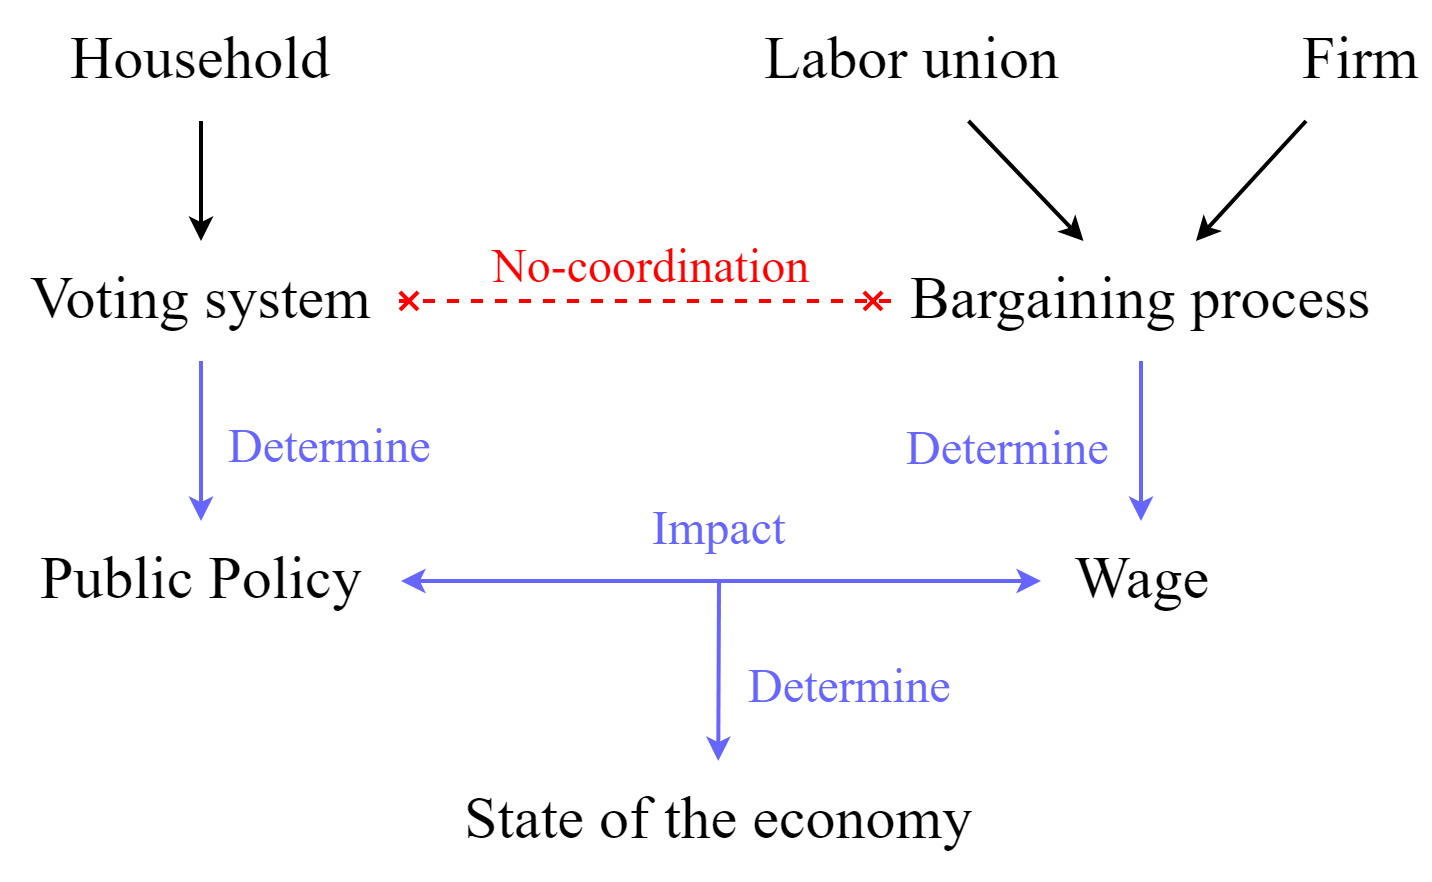
\includegraphics[width=\linewidth]{Diagrams/model_diagram.png}
			\end{figure}
		\end{frame}
		\subsection{Public policy preferences}
			\begin{frame}\frametitle{Public policy preferences}
				\begin{itemize}
					\item Age-related conflict in the public policy :
					\begin{itemize}
						\item Young households desire more unemployment benefit ($b$)
						\item Old households desire more health spending ($h$)
						\item Both desire less taxes ($\tau$)
					\end{itemize}
				\end{itemize}
				\begin{itemize}
					\item Government budget constraint :
						\begin{equation*}
						\tau_t Y_t = b_t u_t N^y_t + h_t N^o_t
						\end{equation*}
				\end{itemize}
				\begin{itemize}
					\item Political objective function :
						\begin{equation*}
						W_t(.) = \omega\left\lbrace u_{t-1}N_t^o U_t^{o,u} + (1-u_{t-1}) N_t^o U_t^{o,e} \right\rbrace + N_t^y \left\lbrace\mathbb{E}\left(U^y_t\right)\right\rbrace
						\end{equation*}
					$\omega \geq 0$ the per-capita relative political influence of old agents
				\end{itemize}
			\end{frame}
			\begin{frame}
				\begin{itemize}
					\item Maximization program characterizing equilibrium policy choices in period $t$ :
				\end{itemize}
					\begin{align*}
						\max_{\lbrace\tau_t, b_t, h_t\rbrace\geq 0} &\ln(1-\tau_t) +\beta \ln h_t + \textcolor{red}{\eta_t} \ln\left[(1-u_t)(1-\tau_t)w_t + u_t b_t\right] + \dots\\
						\text{s.t.} ~~ &\tau_t Y_t = b_t u_t N_t^y + h_t N_t^o
					\end{align*}
					$\textcolor{red}{\eta_t}$ the weight of the young generation within the social welfare function :\\
					\begin{equation*}
						\textcolor{red}{\eta_t} = \frac{n_t}{p_t}\frac{1+\alpha p_{t+1}}{\omega}
					\end{equation*}
			\end{frame}
			\begin{frame}
				\begin{itemize}
					\item Focusing on the interior solution, first order conditions give :
						\begin{align*}
						\frac{b_t}{(1-\tau_t)w_t} &= \frac{1-u_t}{u_t} \left(\textcolor{red}{\eta_t}\frac{1-\theta_t}{\theta_t}- 1\right)\\
						\tau_t &= 1 - \left[\left(1-\theta_t\right)\left(1+\beta+\textcolor{red}{\eta_t}\right)\right]^{-1}\\
						h_t &= \left(\tau_t \frac{Y_t}{N_t^y} - b_t u_t\right)\frac{n_t}{p_t}
						\end{align*}
				\end{itemize}
			\end{frame}	
		\subsection{Wage bargaining}
			\begin{frame}\frametitle{Wage bargaining}
				\begin{itemize}
					\item Right-to-manage model \textit{à la} Nickell \& Andrews (1983) :
					\begin{itemize}
						\item Single union that represents workers and bargains only over wages
						\item Employer retains the prerogative to hire and fire
					\end{itemize}
				\end{itemize}
				\vspace{1em}
				\begin{itemize}
					\item Maximization program characterizing equilibrium wage bargaining :
					\begin{align*}
						\max_{w_t>0} ~~ &\lbrace \left(L_t[U^{y,e}_t - U^{y,u}_t]\right)^\gamma \left(Y_t-w_tL_t\right)^{1-\gamma}\rbrace,~~\gamma\in(0,1)\\
						\text{s.t.} ~~ &U_t^{y,e} - U_t^{y,u} = (1+\alpha p_{t+1})\ln\left[\frac{(1-\tau_t)w_t}{b_t}\right]
					\end{align*}
				\end{itemize}				
			\end{frame}
			\begin{frame}
				\begin{itemize}
%					\item First order condition (FOC) :
%					\begin{equation*}
%						\frac{\gamma}{1-\gamma}\left\lbrace\mathcal{E}^{L,w}_t\ln\left[\frac{(1-\tau_t)w_t}{b_t}\right]+1\right\rbrace = \ln\left[\frac{(1-\tau_t)w_t}{b_t}\right] \frac{\theta_t}{1-\theta_t}
%					\end{equation*}
					\item From the first-order condition :
					\begin{equation*}
						k_t(X_t) = \left[\frac{1-\phi}{\phi}\frac{1-\gamma(1-\sigma)}{\gamma}\frac{X_t}{1-\sigma X_t}\right]^{\frac{\sigma}{\sigma-1}}
					\end{equation*}
					where $X_t=\ln\left[\frac{(1-\tau_t)w_t}{b_t}\right]$ is the value-added to be employed in utility terms.
				\end{itemize}
			\end{frame}
		\subsection{Equilibrium}
			\begin{frame}[label = captolab]\frametitle{Equilibrium}
				\begin{itemize}
					\item Using first order conditions from the voting and wage bargaining, the \textbf{capital-to-labor ratio $(k)$ at the equilibrium} solves :
					\begin{align}
						X_t &= \ln\left( \frac{ \frac{N_t^y}{K_t} k_t - 1 } { \frac{\phi}{1-\phi} k_t^{\frac{\sigma-1}{\sigma}} \eta_t - 1 }\right) \label{eq:x1} \\
						X_t &= \left( \sigma + \frac{1-\phi}{\phi} \frac{1-\gamma(1-\sigma)}{\gamma} k_t^{\frac{1-\sigma}{\sigma}} \right)^{-1} \label{eq:x2}
					\end{align}
					\item Uniqueness of the equilibrium : \hyperlink{uniqueness<1>}{\beamergotobutton{Details}}
				\end{itemize}
			\end{frame}
			\begin{frame}\frametitle{Comparative statics : public policy and households}
				\begin{itemize}
					\item The longer you expect to live, the more you save : $\frac{\partial S_t}{\partial p_{t+1}} > 0$
					\vspace{1em}
					\item Young households desire...
					\begin{itemize}
						\item more redistribution : $\frac{\partial \tau_t}{\partial \eta_t} > 0$
						\item a higher unemployment replacement rate : $\frac{\partial \frac{b_t}{(1-\tau_t)w_t}}{\partial \eta_t}>0$
					\end{itemize}
					\vspace{1em}
					\item Unemployment benefits increases the labor income share : $\frac{\partial \theta_t}{\partial b_t} > 0$
				\end{itemize}
			\end{frame}
			\begin{frame}\frametitle{Comparative statics : labor share}
					\begin{itemize}
						\item Labor share : $\theta_t = \frac{w_t L_t}{Y_t}=  \left(1+\frac{\phi}{1-\phi}k_t^{\frac{\sigma-1}{\sigma}}\right)^{-1}$
						\item Comparative statics :
						\begin{equation*}
							\left\lbrace ~~
							\frac{\partial w_t}{\partial k_t} > 0,~~
							\frac{\partial (Y_t/L_t)}{\partial k_t} > 0,~~
							\frac{\partial \theta_t}{\partial k_t} \lessgtr 0 ~~
							\right\rbrace, ~~ \sigma \gtrless 1
						\end{equation*}
						\item It implies that :
						\begin{equation*}
							\left\lbrace ~~
							\frac{\partial w_t}{\partial k_t} ~\lessgtr~ \frac{\partial (Y_t/L_t)}{\partial k_t} ~~
							\right\rbrace, ~~ \sigma \gtrless 1
						\end{equation*}
						\item Finally,
						\begin{equation*}
							\frac{\partial \theta_t}{\partial X_t} < 0,~~ \forall \sigma \in \mathbb{R}^\star_+ \smallsetminus\lbrace 1 \rbrace
						\end{equation*}
					\end{itemize}
			\end{frame}
	
	\section{Quantitative analysis}
		\subsection{Calibration}
			\begin{frame}\frametitle{Calibration}
				\begin{itemize}
					\item Objectives :
					\begin{enumerate}
						\setbeamertemplate{enumerate items}[default]
						\item Match the labor share dynamics over the period 1970 to 2010
						\item Model prediction over the period 2010 to 2080
					\end{enumerate}
				\end{itemize}
				\vspace{1em}
				\begin{itemize}
					\item Period length : 40 years
					\item Four sequences of model prediction :
					\begin{itemize}
						\item 1\textsuperscript{st} sequence : 1970, 2010, 2050, \dots
						\item 2\textsuperscript{nd} sequence : 1980, 2020, 2060, \dots
						\item 3\textsuperscript{rd} sequence : 1990, 2030, 2070, \dots
						\item 4\textsuperscript{th} sequence : 2000, 2040, 2080, \dots
					\end{itemize}
				\end{itemize}
			\end{frame}
		
			\begin{frame}[label = paraminit]\frametitle{Parameters}
				\begin{center}
					\resizebox{10cm}{!}{	\begin{threeparttable}
		\begin{tabular}{cllc}
			\multicolumn{2}{c}{\textbf{Parameter}}                             & \textbf{Method}   & \textbf{Target}                   \\ \hline
			\hline \\[-1.8ex] 
			$\phi$             & Capital share in 1970                           & Data     & $1-\hat{\theta}_{1970}$             \\ \hline \\[-1.8ex] 
			$\gamma$           & Relative bargaining power of the union          & Fixed    & 0.5                               \\
			$\alpha$           & Discount rate                                   & Fixed    & 0.699                             \\
%			$\tilde{K}_{1970}$ & Initial capital stock                           & Fixed    & 1                                 \\
%			$\tilde{L}_{1970}$ & Initial labor                                   & Fixed    & 1                                 \\
%			$\tilde{k}_{1970}$ & Initial capital-labor ratio                     & Fixed    & 1                                 \\
			 \hline \\[-1.8ex]
			$\sigma$ 		   & Capital-labor elasticity of substitution & \multicolumn{2}{l}{\begin{tabular}[c]{@{}l@{}}Estimate using León-Ledesma,\\McAdam \& Willman (2013, AER)\end{tabular}} \\ \hline \\[-1.8ex]
%			$N_{1970}^y$       & Initial young households                        & Matches  & $\hat{u}_{1970}$                  \\
%			$N_{1970}^o$       & Initial old households                          & Matches  & $\hat{p}_{1970} / \hat{n}_{1970}$ \\
			$\omega$           & Relative per-capita influence of old households & Matches  & $\hat{k}_{1970}$                  \\
			$\beta$            & Preference for government health expenditure    & Matches  & $\hat{\tau}_{1970}$               \\
			$A$                & Scale parameter of the production function 	 & Matches  & $\hat{\theta}_{2010}$             \\ \hline
			\hline
		\end{tabular}
		\begin{tablenotes}
			{\footnotesize 
			\item \textit{Note :} Initial variables are normalized to 1970. Variables with hat are from data. ``Matches'' refers to ``\textit{set such that the model prediction matches the target}''. Data from Penn World Table 9.0, World Population Prospect (United Nations) and OECD database.
			}
		\end{tablenotes}
	\end{threeparttable}}
				\end{center}
				\hyperlink{leon<1>}{\beamergotobutton{León-Ledesma, McAdam \& Willman (2013, AER)}}
			\end{frame}
		
			\begin{frame}
				\begin{center}
					\resizebox{10cm}{!}{\begin{table}[tb]
	\caption{Parameters}\label{tab:param}
	\centering
	\begin{threeparttable}
		\begin{tabular}{c l D{.}{.}{-3} D{.}{.}{-3}}
			\multicolumn{2}{c}{\textbf{Parameter}} & \multicolumn{1}{r}{\textbf{France}} & \multicolumn{1}{r}{\textbf{United States}}            \\ \hline \hline
			$\phi$             & Capital share in 1970                           & 0.27 & 0.325		\\ \hline
			$\gamma$           & Relative bargaining power of the union          & 0.5 & 0.5				\\ [-1ex]
			$\alpha$           & Discount rate                                   & 0.669 & 0.669		\\ \hline
			$\sigma$           & Capital-labor elasticity of substitution        & 1.279 & 1.234	\\ \hline
			$\omega$           & Relative ideological spread-out				 & 0.983 & 1.533		\\ [-1ex]
			$\beta$            & Preference for government health expenditure    & 0.739 & 0.138		\\ [-1ex]
			$A$                & Scale parameter of the production function		 & 28.23 & 22.84				\\ \hline \hline
		\end{tabular}
		\vspace{-3ex}
		\begin{tablenotes}
			{\singlespacing\footnotesize
				\item \textit{Note :} Single-equation estimation of $\sigma$ from the two first-order conditions of the profit maximization with normalized CES production function. $\sigma$ estimates are significant at $p<0.1$ for France and $p<0.05$ for the United States. Details in \hyperref[appendix:sigma]{appendix C}.
			}
		\end{tablenotes}
	\end{threeparttable}
\end{table}}
				\end{center}
			\end{frame}		
			\subsection{Model prediction}
			\begin{frame}\frametitle{Labor share : data versus model prediction}
				\begin{figure}[h]
					\begin{subfigure}[h]{0.49\linewidth}
						\centering
						\begin{overlayarea}{\textwidth}{\textheight}
							\only<1>{\includegraphics[width=\textwidth]{Figures/FRDM1.png}
								\caption{France}}
							\only<2>{\includegraphics[width=\textwidth]{Figures/FRDM2.png}
								\caption{France}}
						\end{overlayarea}
					\end{subfigure}
					%%%
					\begin{subfigure}[h]{0.49\linewidth}
						\centering
						\begin{overlayarea}{\textwidth}{\textheight}
							\only<1>{\includegraphics[width=\textwidth]{Figures/USDM1.png}
								\caption{United States}}
							\only<2>{\includegraphics[width=\textwidth]{Figures/USDM2.png}
								\caption{United States}}
						\end{overlayarea}
					\end{subfigure}
					%\caption{Labor share : data versus model prediction}
					%\label{fig:LS7010} 
				\end{figure}
			\end{frame}
		\subsection{Demographic effects decomposition}
			\begin{frame}\frametitle{Demographic effects decomposition}
			\begin{itemize}
				\item (Reminder) Old-age dependency ratio : 
				\begin{equation*}
				\frac{N_t^o}{N_t^y} = \frac{p_t}{n_t}
				\end{equation*}
				\item Aging is due to two phenomena :
				\begin{enumerate}
					\setbeamertemplate{enumerate items}[default]
					\item Declining population growth : $n_t\searrow$
					\item Increasing survival rate : $p_t\nearrow, ~  p_{t+1}\nearrow$
				\end{enumerate}
				\item Through two channels :
				\begin{enumerate}
					\setbeamertemplate{enumerate items}[default]
					\item Direct cohort effect : $n_t, ~p_t, ~p_{t+1}$
					\item Indirect cohort effect : $\eta(n_t, p_t, p_{t+1})$
				\end{enumerate}
			\end{itemize}
			\end{frame}
			\begin{frame}\frametitle{Labor share in France : counterfactual (2010)}
				\begin{figure}[h]
					\centering
					\begin{overlayarea}{\textwidth}{\textheight}
						\only<1>{\includegraphics[width=\textwidth]{Figures/FR_SRPG2_2010_large.png}}
						\only<2>{\includegraphics[width=\textwidth]{Figures/FR_SRPG3_2010_large.png}}
						\only<3>{\includegraphics[width=\textwidth]{Figures/FR_SRPG4_2010_large.png}}
						\only<4>{\includegraphics[width=\textwidth]{Figures/FR_SRPG5_2010_large.png}}
						\label{fig:FR_2010_large}
					\end{overlayarea}
				\end{figure}
			\end{frame}
			\begin{frame}\frametitle{Labor share in France : counterfactual (1970)}
				\begin{figure}[h]
					\centering
					\begin{overlayarea}{\textwidth}{\textheight}
						\includegraphics[width=\textwidth]{Figures/FR_SRPG5_1970_large.png}
						\label{fig:FR_SRPG_1970_large}
					\end{overlayarea}
				\end{figure}
			\end{frame}
			\begin{frame}\frametitle{Aging-effect decomposition : sources}
				\begin{figure}[h]
					\centering
					\begin{overlayarea}{\textwidth}{\textheight}
						\includegraphics[width=\textwidth]{Figures/FR_SRPG_1970_large.png}
						\label{fig:FR_SRPG_decomp_1970}
					\end{overlayarea}
				\end{figure}
			\end{frame}
%			\begin{frame}\frametitle{Labor share in France : counterfactual (1970)}
%				\begin{figure}[h]
%					\centering
%					\begin{overlayarea}{\textwidth}{\textheight}
%						\includegraphics[width=\textwidth]{Figures/FR_DEIE5_1970_large.png}
%						\label{fig:FR_DEIE_1970_large}
%					\end{overlayarea}
%				\end{figure}
%			\end{frame}
			\begin{frame}\frametitle{Aging-effect decomposition : transmission channels}
				\begin{figure}[h]
					\centering
					\begin{overlayarea}{\textwidth}{\textheight}
						\includegraphics[width=\textwidth]{Figures/FR_DEIE_1970_large.png}
						\label{fig:FR_DEIE_decomp_1970}
					\end{overlayarea}
				\end{figure}
			\end{frame}
		\subsection{Discussion}
			\begin{frame}\frametitle{Baby-boomer generation in France}
				\begin{minipage}[h]{.49\textwidth}
					\begin{itemize}
						\item When they were young :
						\begin{itemize}
							\item \textbf{Direct effect} : increased savings ($K_{t+1} \nearrow$) and labor supply ($N^y_t \nearrow$)
							\item \textbf{Indirect effect} : increased the outside option of workers ($w_t \nearrow ~ \Rightarrow ~ L_t \searrow$)
							%						\item Substitution between $K$ and $L$ (i.e. $\sigma > 1$) : reduced the labor share.
						\end{itemize}
						\item Nowadays they are old :
						\begin{itemize}
							\item \textbf{Indirect effect} : reduces the outside option of workers ($w_t \searrow ~ \Rightarrow ~ L_t \nearrow$)
						\end{itemize}
					\end{itemize}
				\end{minipage}
				\begin{minipage}[h]{.49\textwidth}
					\includegraphics[width=\textwidth]{Figures/FRDM2.png}
				\end{minipage}
%				\begin{itemize}
%					\item Became young active between 1965 and 1985 and should retire between 2005 and 2025.
%					\item Labor income share : $\theta_t = \frac{w_t L_t}{Y_t}$
%					\begin{itemize}
%						\item $\left\lbrace ~~
%						\frac{\partial w_t}{\partial k_t} ~\leq~ \frac{\partial (Y_t/L_t)}{\partial k_t} ~~
%						\right\rbrace, ~~ \sigma > 1$
%					\end{itemize}
%				\end{itemize}
			\end{frame}
				
	\section{Conclusion}
		\begin{frame}\frametitle{Conclusion}
			\begin{itemize}
				\item OLG Model able to \textbf{link the labor share to demographic dynamics} : through
				\begin{itemize}
					\item Age-related conflict within public policy
					\item Wage bargaining
				\end{itemize}
				\vspace{1em}
				\item Biased technical change is a response of firms to \textbf{income share \textit{grability} of workers} {\footnotesize (Caballero \& Hammour, 1998)}
				\item Demographic dynamics may be a determinant of this \textit{grability} and thus be the source of the bias
			\end{itemize}
		\end{frame}

	\appendix
	\section*{Appendix}
		\begin{frame}[label = preferences]\frametitle{Preferences}
			\begin{itemize}
				\item Household maximization program :
				\begin{align*}
					\max_{\lbrace c_{1,t}, c_{2,t+1} \rbrace \geq 0} &\ln(c_{1,t}) + \alpha p_{t+1}\left\lbrace \ln(c_{2,t+1}) + \beta \ln(h_{t+1}) \right\rbrace\\
					\text{s.t.} ~~ & \begin{cases}
					c_{1,t} + s_t = y_t \\
					c_{2,t+1} = (1-\tau_{t+1}) s_t \hat{R}_{t+1}
					\end{cases}
				\end{align*}
				\item Each young household faces an idiosyncratic unemployment risk with probability $u_t \in \left[0,1\right]$.
				\item Net income of a young household :
				\begin{equation*}
					y_t = \begin{cases}
					(1-\tau_t) w_t ~~ &\text{if employed}\\
					b_t ~~ &\text{if unemployed}
					\end{cases}
				\end{equation*}
			\end{itemize}
			\hyperlink{olgmodel<1>}{\beamerreturnbutton{Return}}
	\end{frame}
	\begin{frame}[label = utilityresult]
		\begin{itemize}
			\item Solving the household maximization program \hyperlink{focutility<1>}{\beamergotobutton{FOC}}, \textbf{aggregate saving} in the economy is :
			\begin{equation*}
				S_t = \frac{\alpha p_{t+1}}{1+\alpha p_{t+1}}\left[ (1-u_t)(1-\tau_t)w_t + u_t b_t \right] N_t^y
			\end{equation*}
			\item Indirect and expected utilities : \hyperlink{indexputility<1>}{\beamergotobutton{Details}}
			\item Gap between between being employed and unemployed in utility terms :
			\begin{equation*}
				U_t^{y,e} - U_t^{y,u} = (1+\alpha p_{t+1})\ln\left[\frac{(1-\tau_t)w_t}{b_t}\right]
			\end{equation*}
		\end{itemize}
		\hyperlink{olgmodel<1>}{\beamerreturnbutton{Return}}
	\end{frame}
	\begin{frame}\frametitle{Production}
		\begin{itemize}
			\item Representative firm with a standard CES production function :
			\begin{equation*}
				Y_t = A\left[ \phi K_t^{\frac{\sigma - 1}{\sigma}} + (1-\phi) L_t^{\frac{\sigma - 1}{\sigma}}\right]^{\frac{\sigma}{\sigma-1}}, ~~ \text{with } \begin{cases}
				\sigma \in \mathbb{R}^\star_+ \smallsetminus\lbrace 1 \rbrace \\
				\phi \in (0,1) \\
				A > 0
				\end{cases} 
			\end{equation*}
			\item Production in units of labor :
			\begin{equation*}
				\frac{Y_t}{L_t} = A\left(\phi k_t^{\frac{\sigma-1}{\sigma}} + 1-\phi\right)^{\frac{\sigma}{\sigma-1}},~~ \text{with } k_t \equiv \frac{K_t}{L_t}
			\end{equation*}
		\end{itemize}
		\hyperlink{olgmodel<1>}{\beamerreturnbutton{Return}}
	\end{frame}
	\begin{frame}\frametitle{Labor demand}
		\begin{itemize}
			\item Labor-demand equation (from profit maximization) :
			\begin{equation*}
				w_t = (1-\phi)A\left(\phi k_t^{\frac{\sigma-1}{\sigma}}+1-\phi\right)^{\frac{1}{\sigma-1}}
			\end{equation*}
			\item Labor-demand elasticity :
			\begin{equation*}
				\mathcal{E}^{L,w}_t = \frac{\partial L_t}{\partial w_t}\frac{w_t}{L_t} = -\sigma\left(1+\frac{1-\phi}{\phi}k_t^{\frac{1-\sigma}{\sigma}}\right)
			\end{equation*}					
		\end{itemize}
		\hyperlink{olgmodel<1>}{\beamerreturnbutton{Return}}
	\end{frame}
		\begin{frame}[label = focutility]
			\begin{itemize}
				\item First order conditions for an $i$-type young household at time $t$ :
				\begin{align*}
				c^i_{1,t} &= \frac{1}{1+\alpha p_{t+1}} y^i_{t} \\
				c^i_{2,t+1} &= \frac{\alpha p_{t+1}}{1+\alpha p_{t+1}}(1-\tau_{t+1})\hat{R}_{t+1}y^i_{t} \\
				s^i_t &= \frac{\alpha p_{t+1}}{1+\alpha p_{t+1}} y^i_t
				\end{align*}
				\item Aggregate saving is :
				\begin{equation*}
					S_t = (1-u_t)N_t^ys_t^e + u_t N_t^y s_t^u
				\end{equation*}
			\end{itemize}
			\hyperlink{utilityresult<1>}{\beamerreturnbutton{Return}}
		\end{frame}
		\begin{frame}[label = indexputility]
			\begin{itemize}
				\item Indirect utility of an $i$-type old household at time $t$ :
				\begin{equation*}
				U_t^{o,i} = \ln\left(\frac{\alpha p_t}{1+\alpha p_t}(1-\tau_t)y_{t-1}^i\hat{R}_t\right) + \beta \ln(h_t) ~~ \forall i = \lbrace e,u \rbrace
				\end{equation*}
				\item Indirect utility of an $i$-type young household at time $t$ :
				\begin{equation*}
				U_t^{y,i} = \ln\left(\frac{1}{1+\alpha p_{t+1}}y_t^i\right)+ \alpha p_{t+1} U_{t+1}^{o,i} ~~ \forall i = \lbrace e,u \rbrace
				\end{equation*}
				\item Expected utility of a young household at time $t$ :
				\begin{align*}
				&\mathbb{E}({U}_t^y) = \ln\left(\frac{1}{1+\alpha p_{t+1}}\mathbb{E}\left(y_t\right)\right) +\\
				&\alpha p_{t+1}\left\lbrace \ln\left(\frac{\alpha p_{t+1}}{1+\alpha p_{t+1}}(1-\tau_{t+1})\mathbb{E}(y_t)\hat{R}_{t+1}\right) + \beta \ln(h_{t+1}) \right\rbrace
				\end{align*}
				\item Expected income of a young household at time $t$ :
				\begin{equation*}
					\mathbb{E}(y_t) = (1-u_t)(1-\tau_t)w_t + u_tb_t
				\end{equation*}			
			\end{itemize}
			\hyperlink{utilityresult<1>}{\beamerreturnbutton{Return}}
		\end{frame}
		\begin{frame}[label = uniqueness]\frametitle{Equation \eqref{eq:x1} analysis}
			\begin{itemize}
				\item \eqref{eq:x1} : $g(k_t) = \ln\left( \frac{\frac{k_t}{k_1}-1}{\left(\frac{k_t}{k_2}\right)^{\frac{\sigma - 1}{\sigma}} - 1} \right), ~~ \text{with }\begin{cases} k_1 &= \frac{K_t}{N_t^y} \\ k_2 &= \left(\frac{1-\phi}{\phi} \frac{1}{\eta_t} \right)^{\frac{\sigma}{\sigma-1}} \end{cases}$
			\end{itemize}
			\begin{figure}[ht]
				\begin{subfigure}[t]{0.24\linewidth}
					\centering
					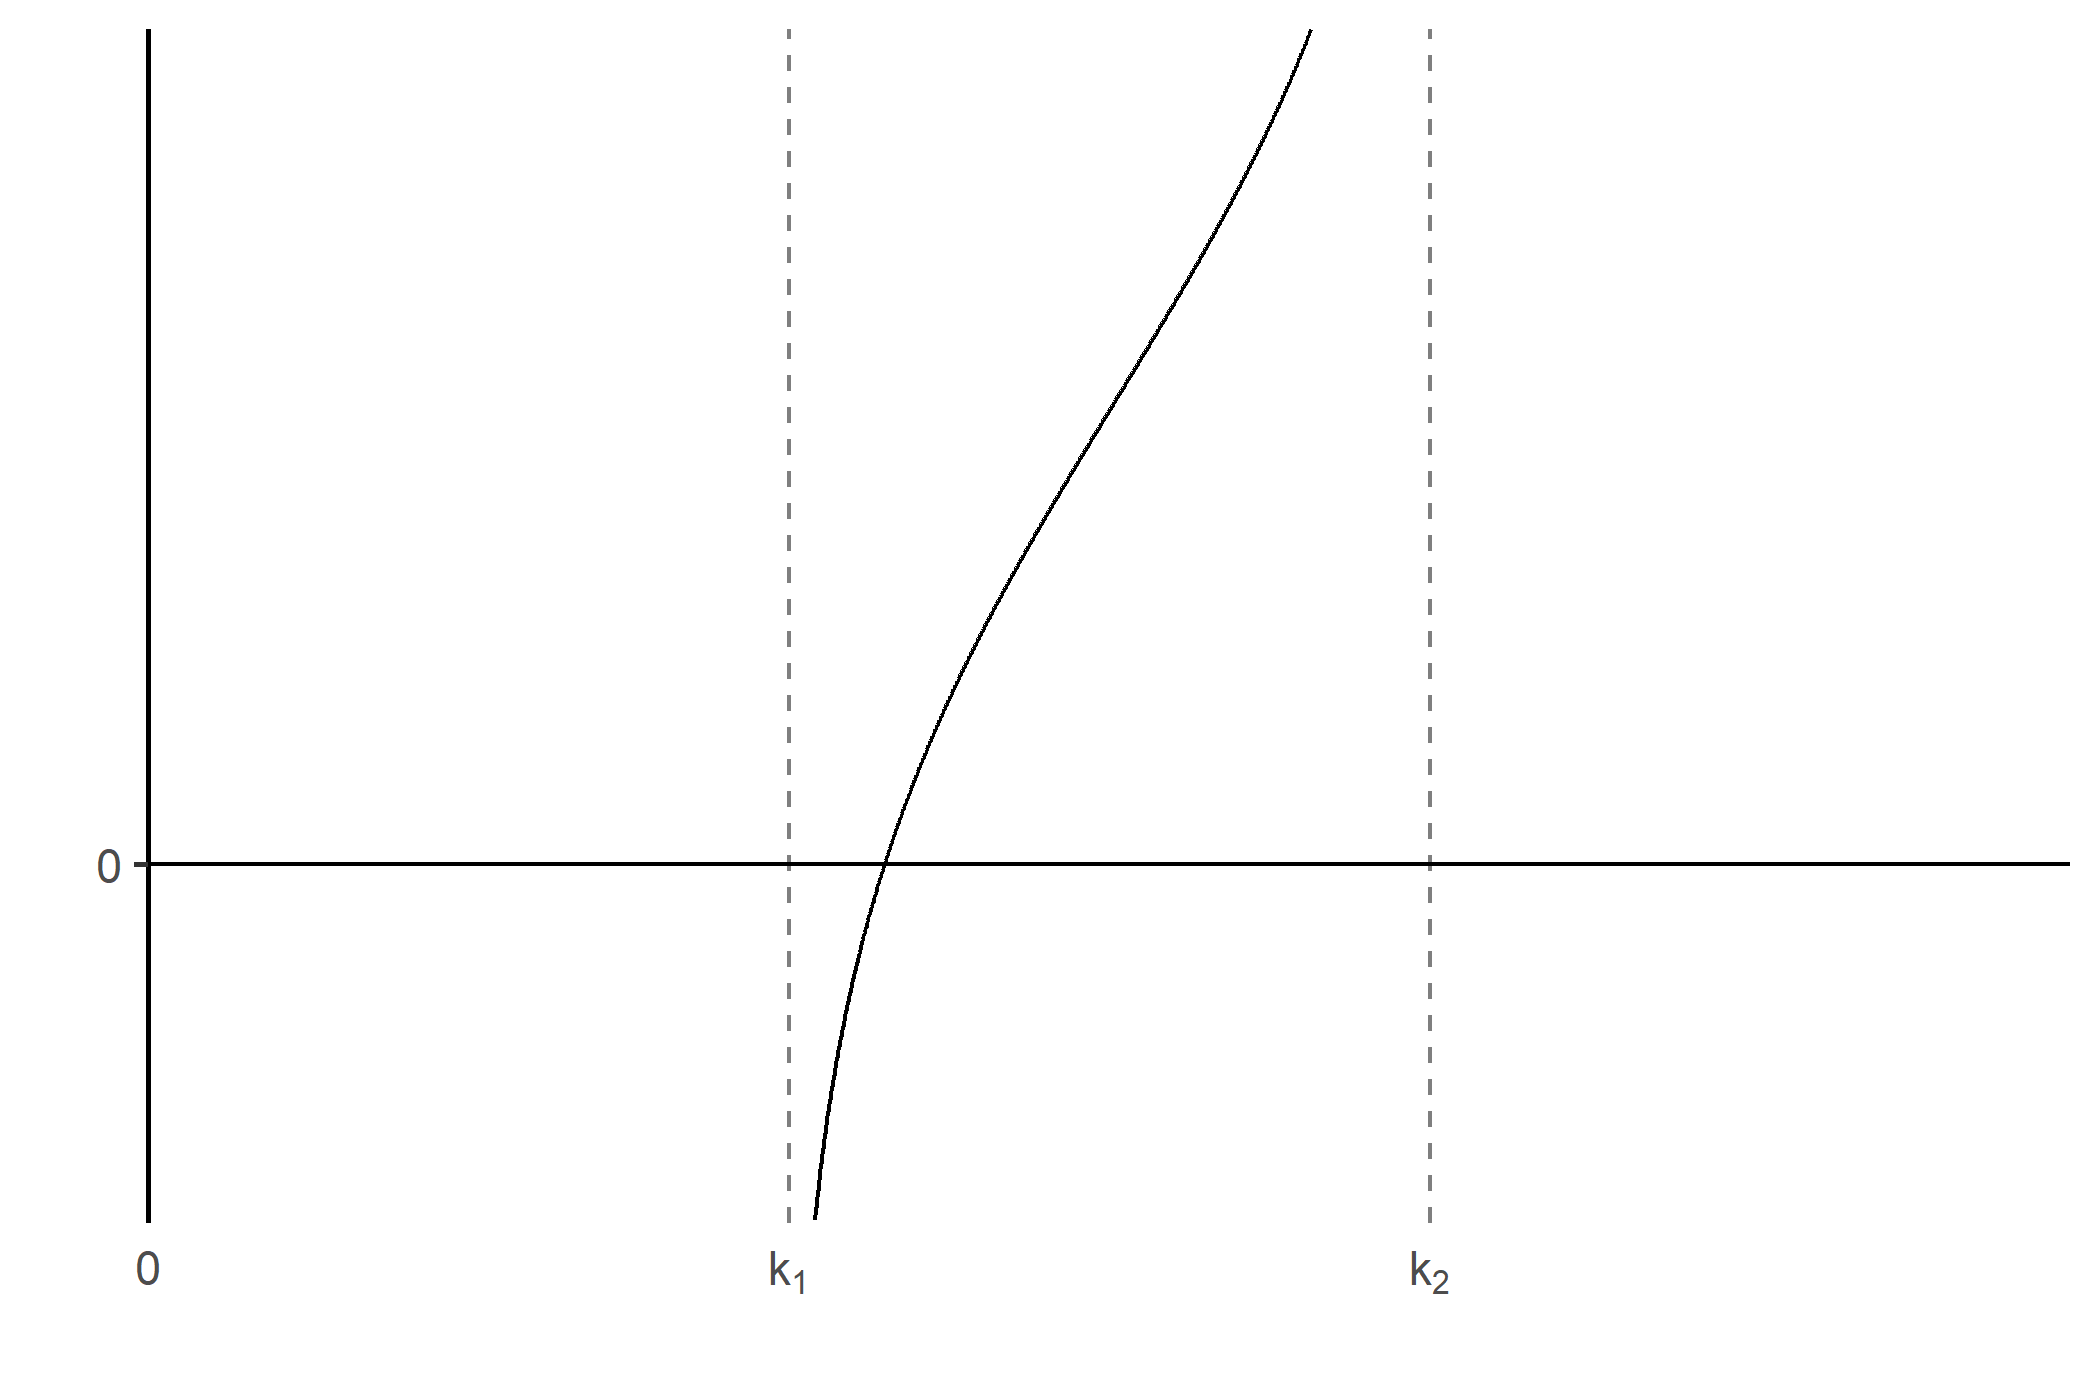
\includegraphics[width=1\linewidth]{Figures/graph_a} 
					\caption{$\begin{cases}
						&\sigma < 1 \\ &k_1 < k_2
						\end{cases}$}
					\label{fig:graph_a}
				\end{subfigure}
				%%%
				\begin{subfigure}[t]{0.24\linewidth}
					\centering
					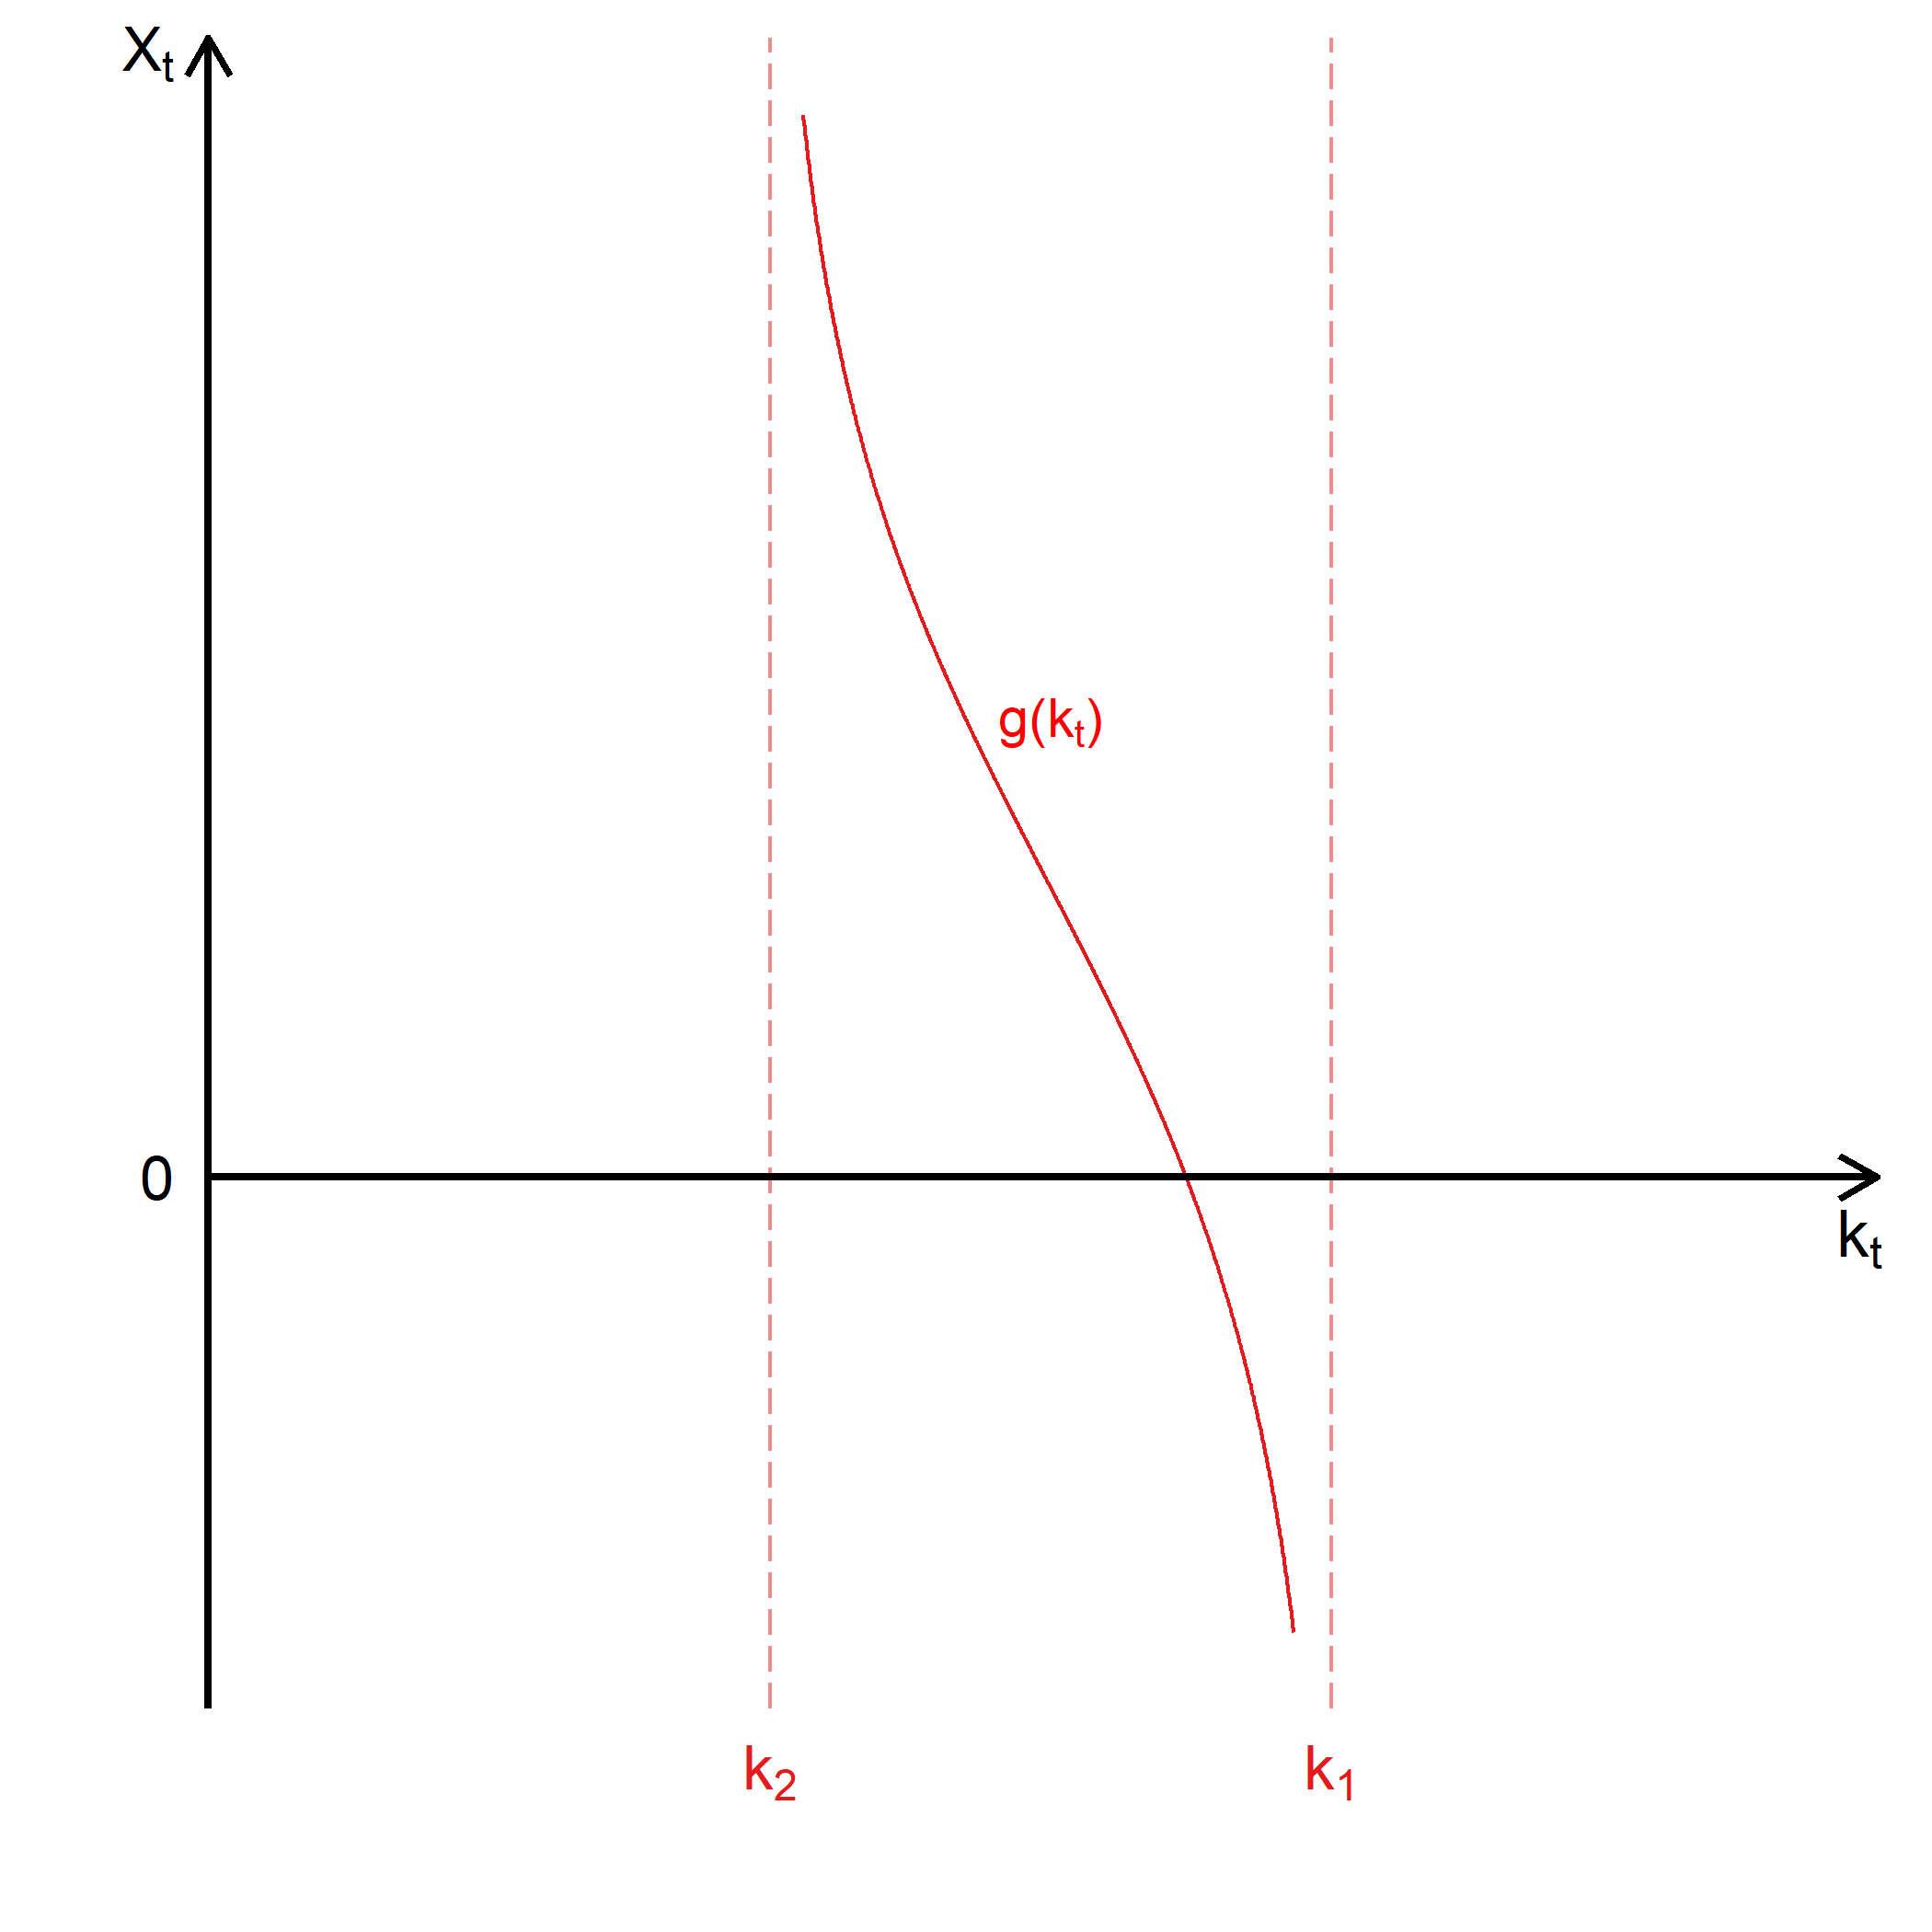
\includegraphics[width=1\linewidth]{Figures/graph_b} 
					\caption{$\begin{cases}
						&\sigma < 1 \\ &k_1 > k_2
						\end{cases}$} 
					\label{fig:graph_b}
				\end{subfigure}
				%%%
				\begin{subfigure}[t]{0.24\linewidth}
					\centering
					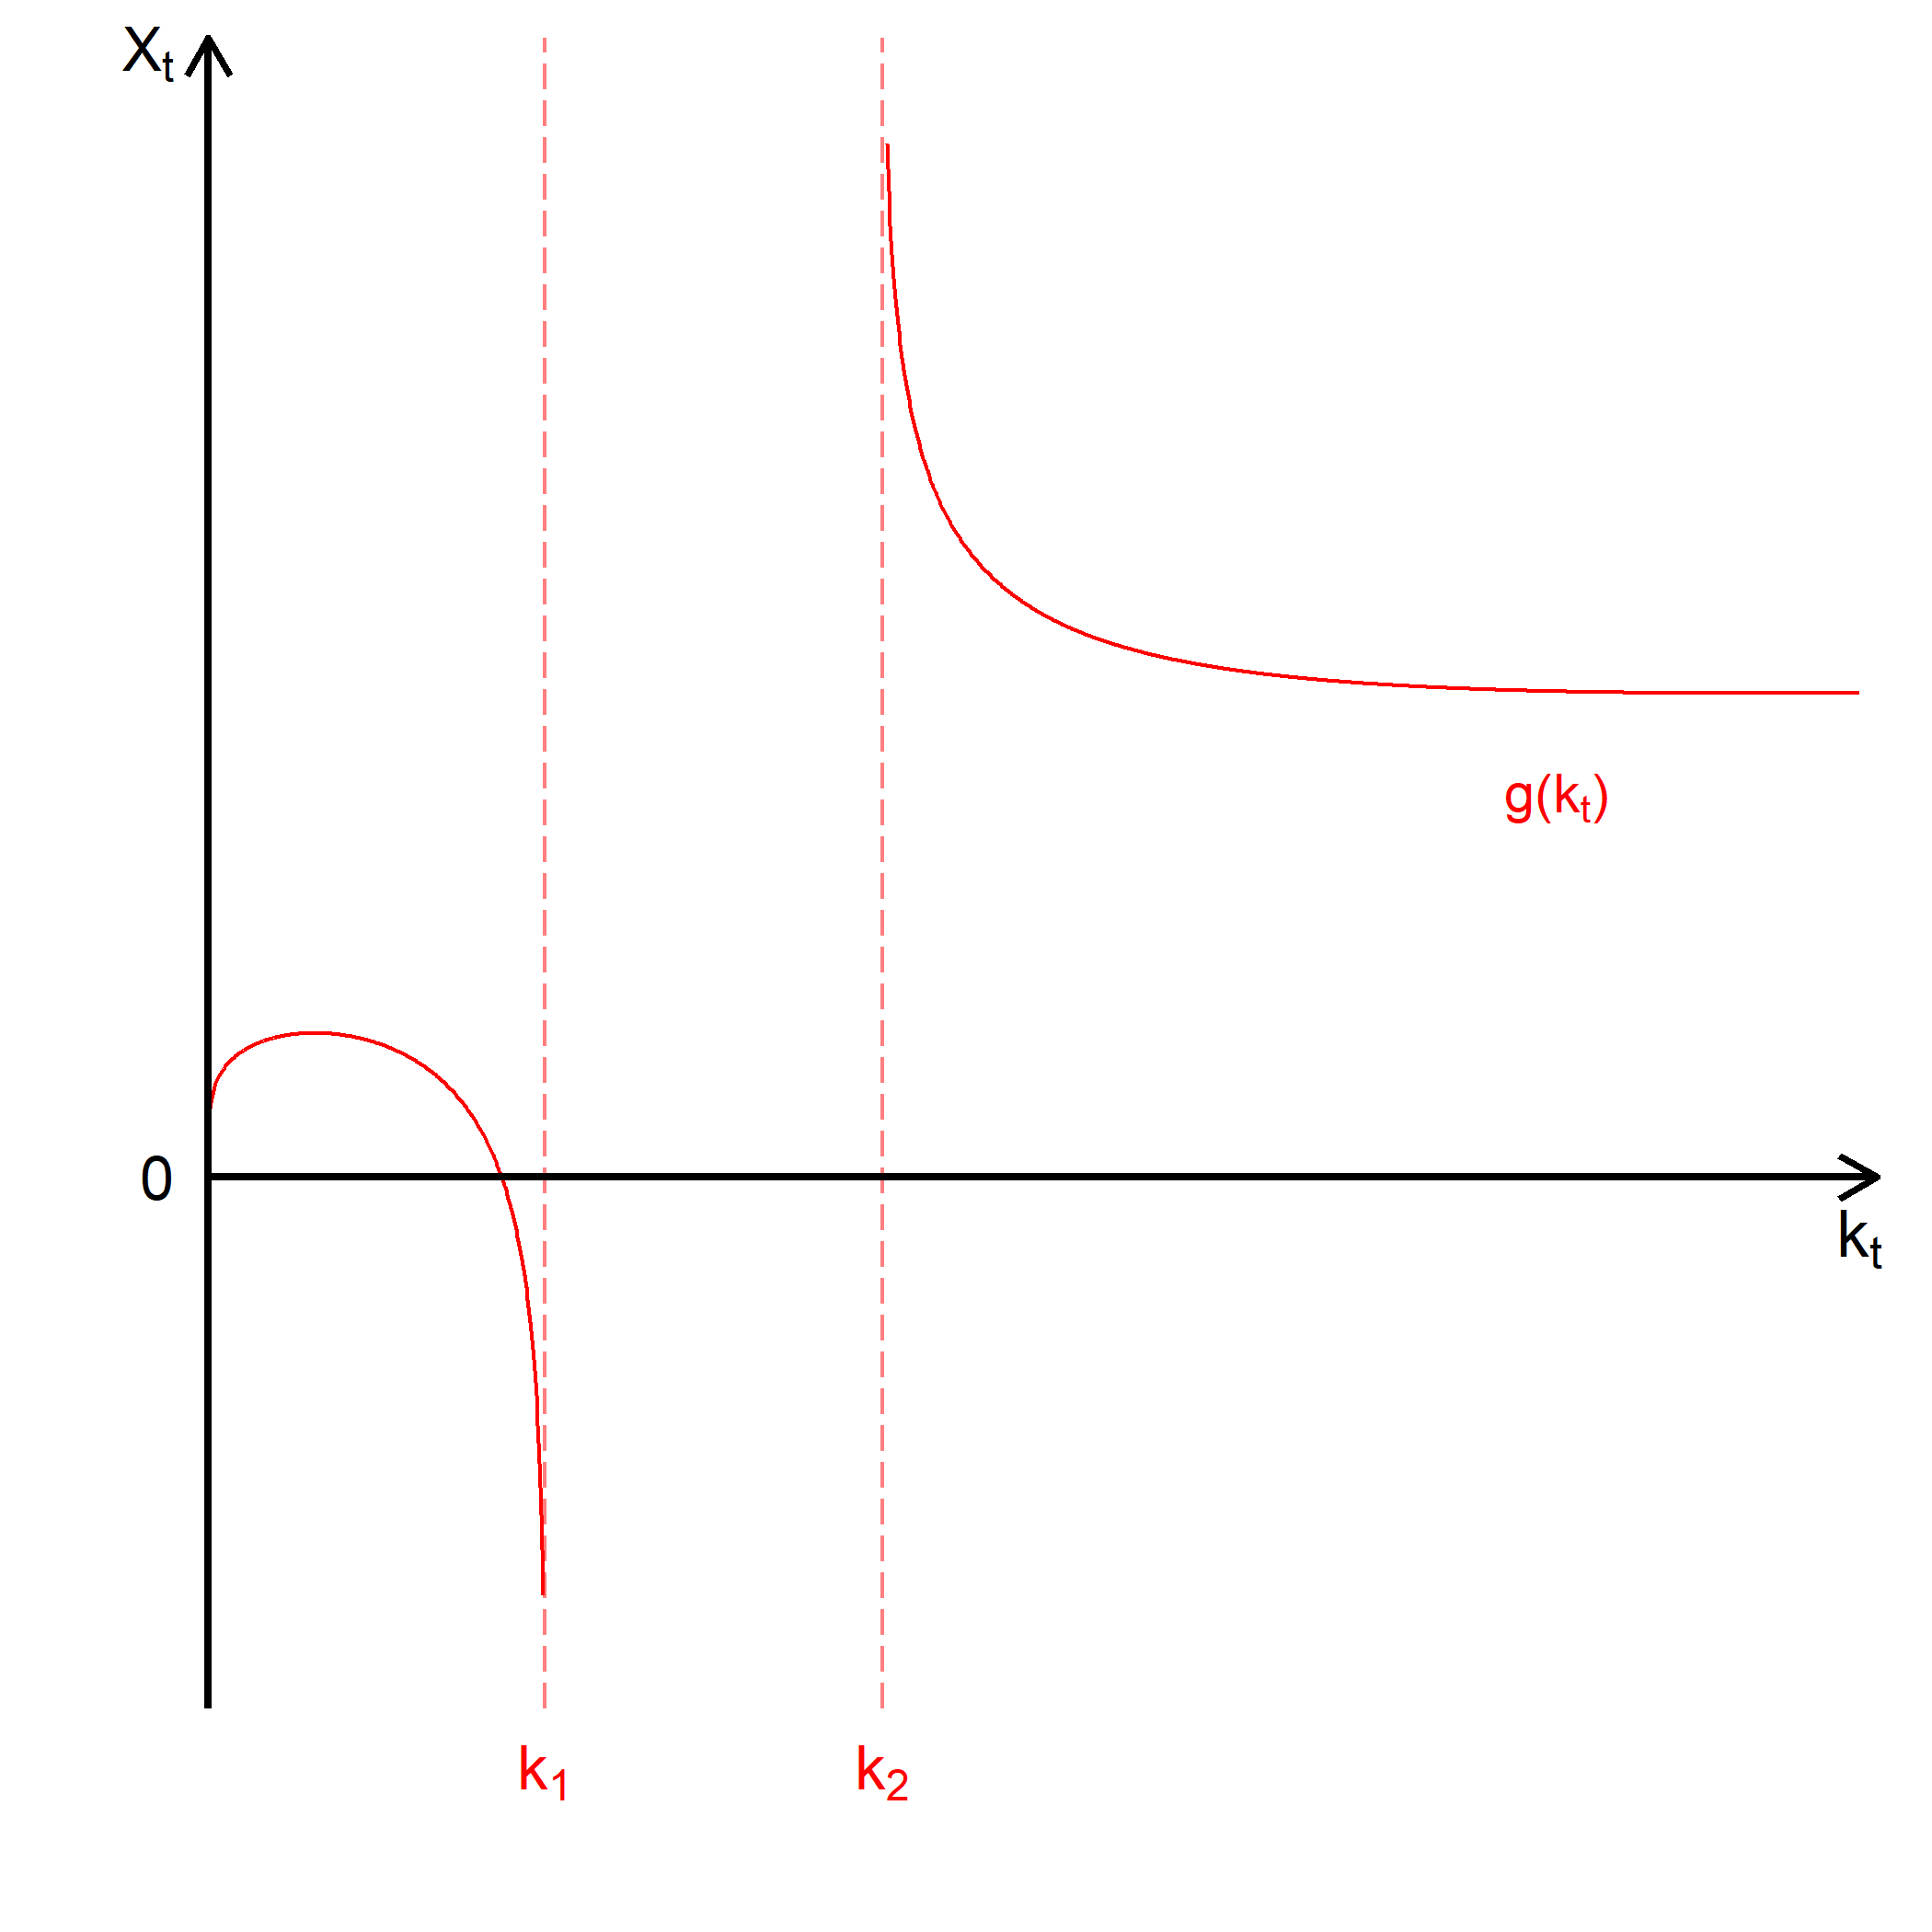
\includegraphics[width=1\linewidth]{Figures/graph_c} 
					\caption{$\begin{cases}
						&\sigma > 1 \\ &k_1 < k_2
						\end{cases}$} 
					\label{fig:graph_c} 
				\end{subfigure}
				%%%
				\begin{subfigure}[t]{0.24\linewidth}
					\centering
					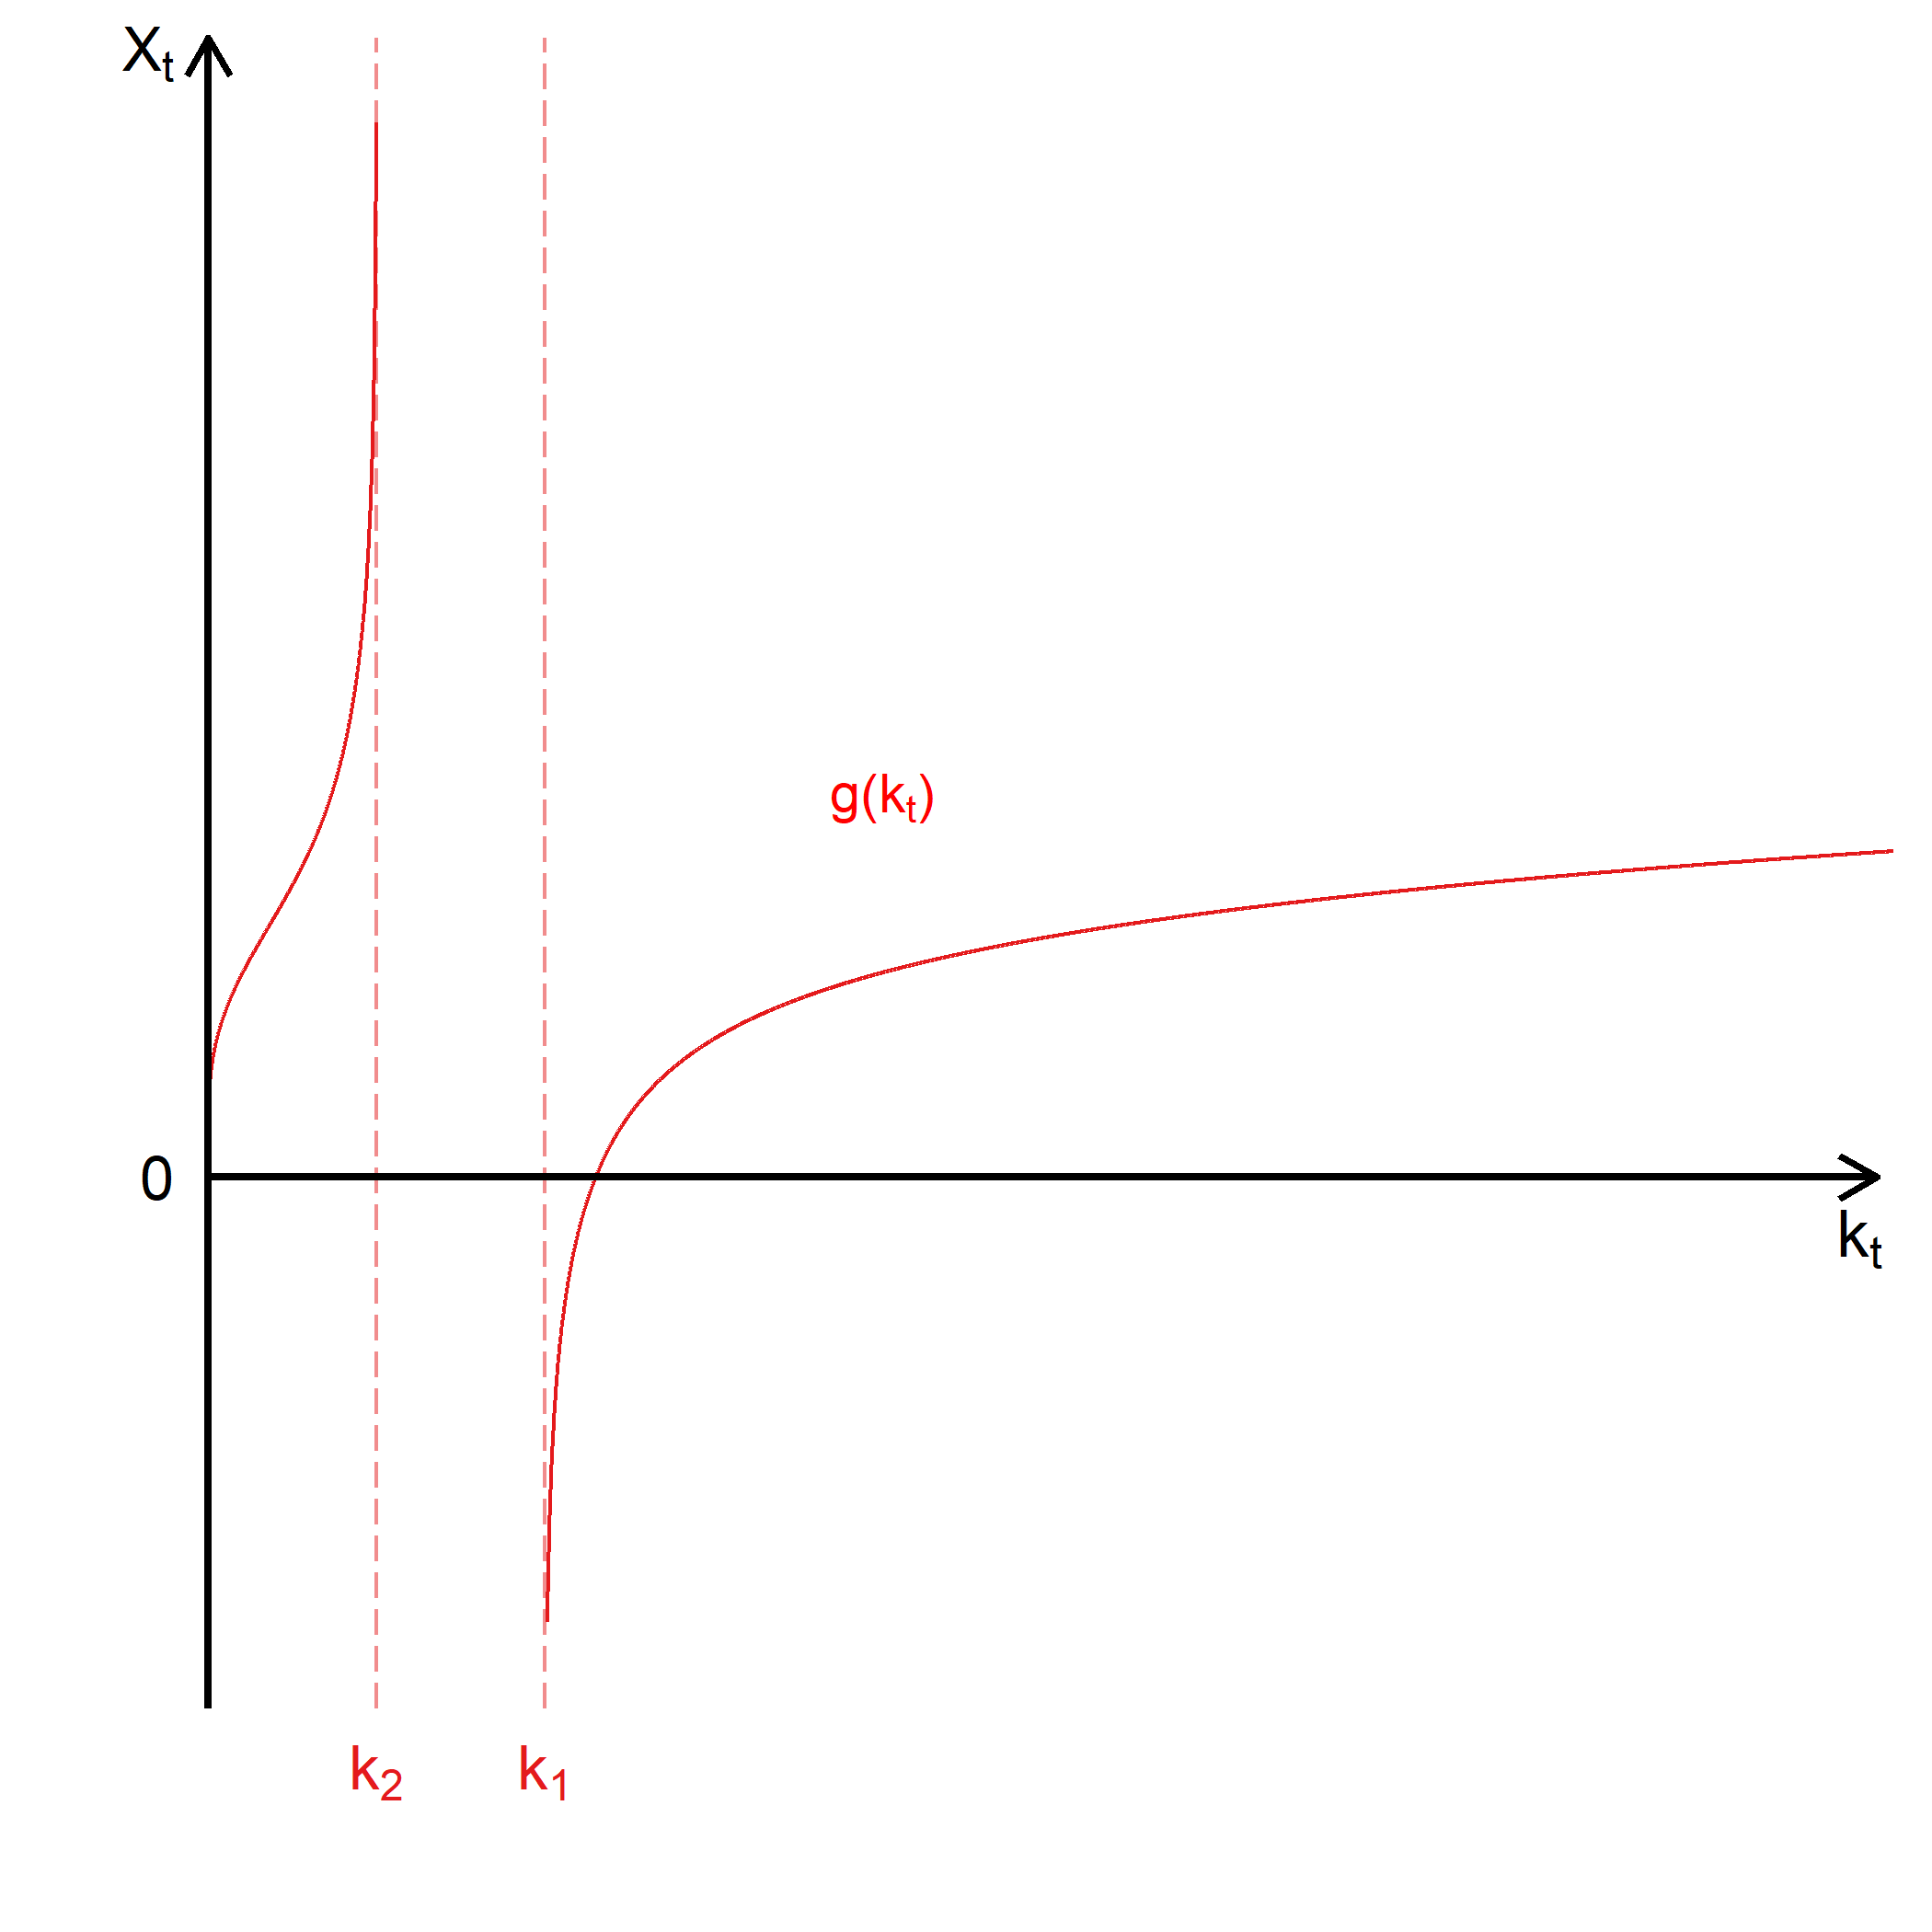
\includegraphics[width=1\linewidth]{Figures/graph_d} 
					\caption{$\begin{cases}
						&\sigma > 1 \\ &k_1 > k_2
						\end{cases}$} 
					\label{fig:graph_d} 
				\end{subfigure}
			\end{figure}
			\hyperlink{captolab<1>}{\beamerreturnbutton{Return}}
		\end{frame}
		\begin{frame}\frametitle{Equation \eqref{eq:x1} analysis}
			\begin{itemize}
				\item Both cases (b) and (c) implies that the labor demand exceeds the labor force
				\item Since the labor supply is inelastic, there is full employment (i.e. $L_t = N_t^y$) and $X_t = 0 \Leftrightarrow (1-\tau_t)w_t = b_t$.
				\vspace{1em}
				\item Thus, we only consider cases (a) and (d) with \eqref{eq:x2}.
				\item $\frac{\partial g}{\partial k_t}(0) = +\infty,~~\text{when }\sigma > 1$
			\end{itemize}
			\hyperlink{captolab<1>}{\beamerreturnbutton{Return}}
		\end{frame}
		\begin{frame}\frametitle{Equation \eqref{eq:x2} analysis}
			\begin{itemize}
				\item \eqref{eq:x2} : $ h(k_t) = \left( \sigma + \frac{1-\phi}{\phi} \frac{1-\gamma(1-\sigma)}{\gamma} k_t^{\frac{1-\sigma}{\sigma}} \right)^{-1}$
			\end{itemize}
			\begin{figure}[ht] 
				\begin{subfigure}[t]{0.32\linewidth}
					\centering
					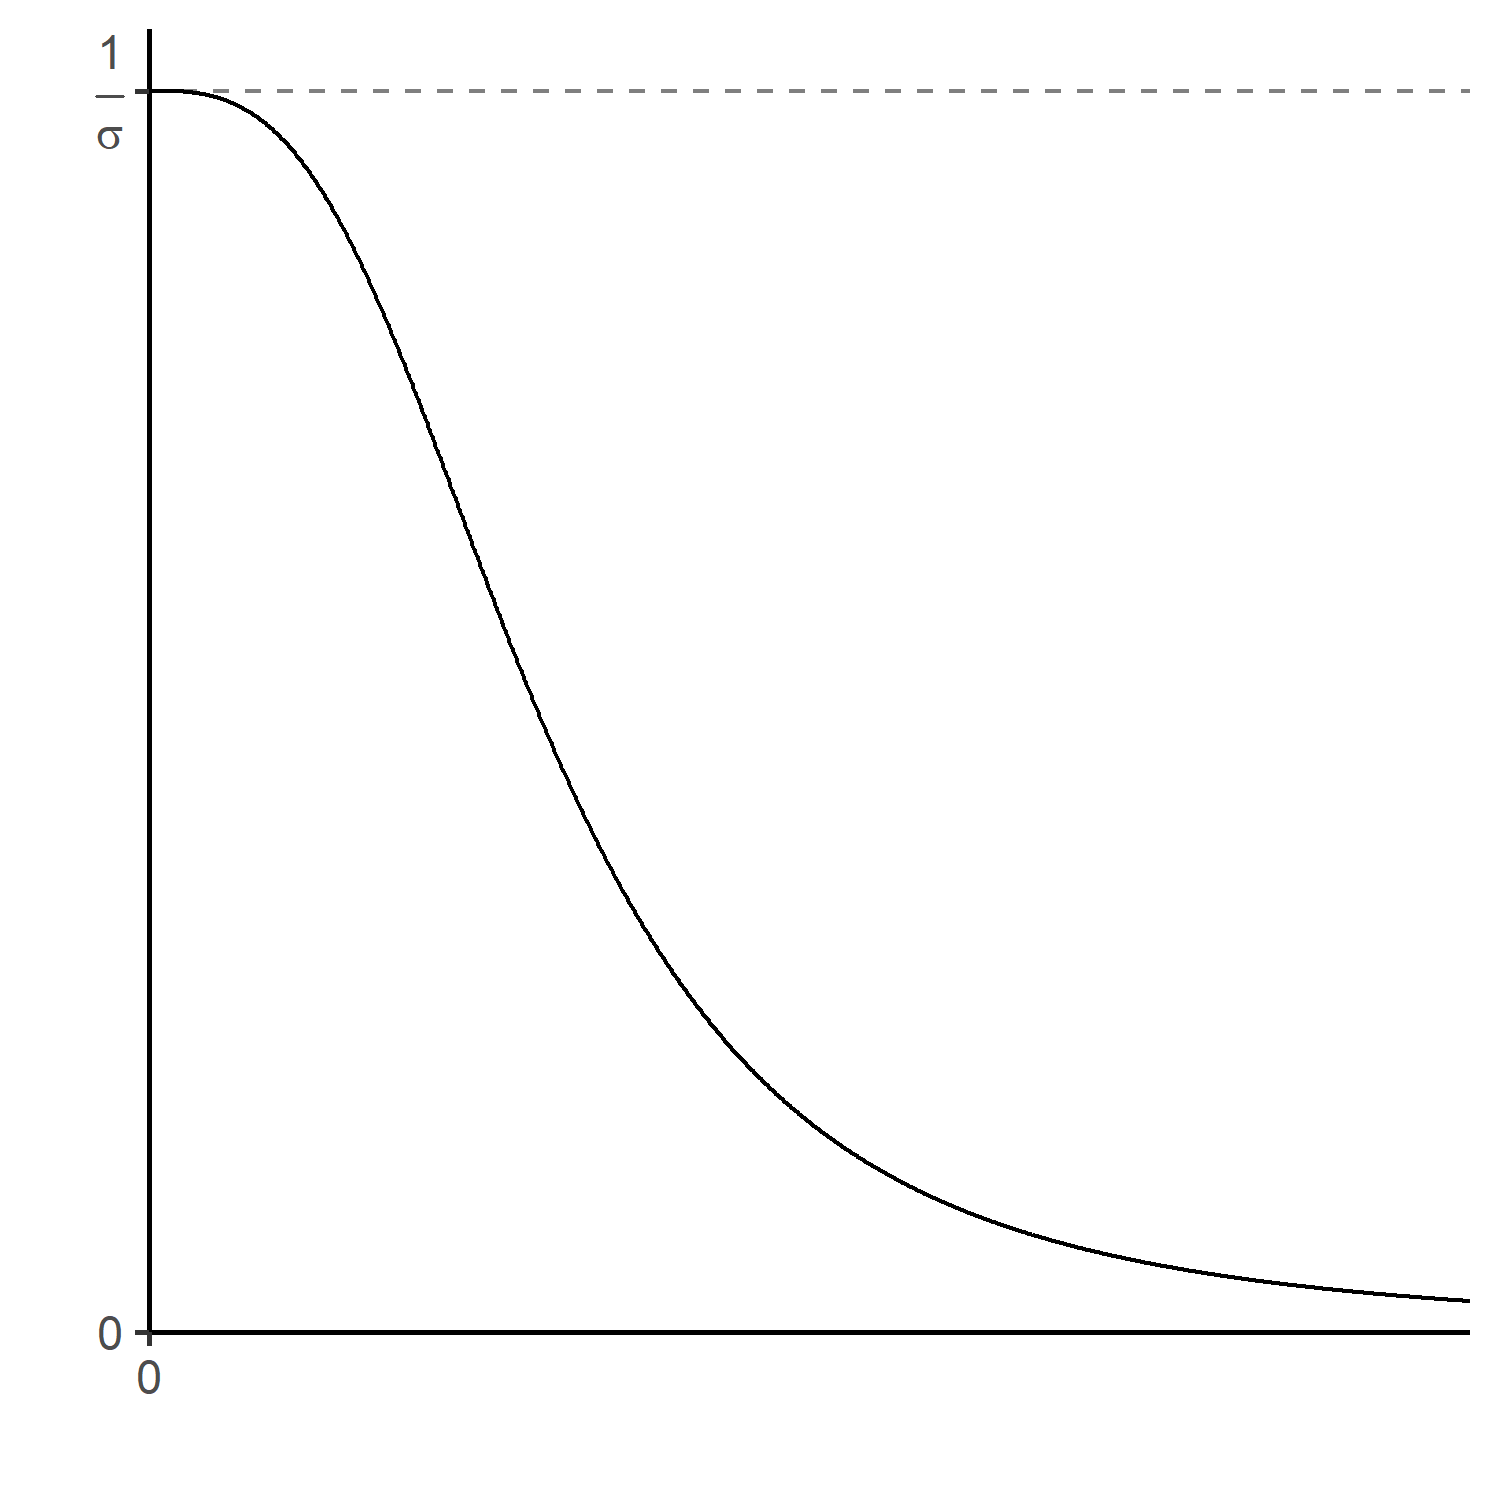
\includegraphics[width=1\linewidth]{Figures/graph_1} 
					\caption{$ \sigma < 0.5$} 
					\label{fig:graph_1} 
					\vspace{4ex}
				\end{subfigure}
				%%%
				\begin{subfigure}[t]{0.32\linewidth}
					\centering
					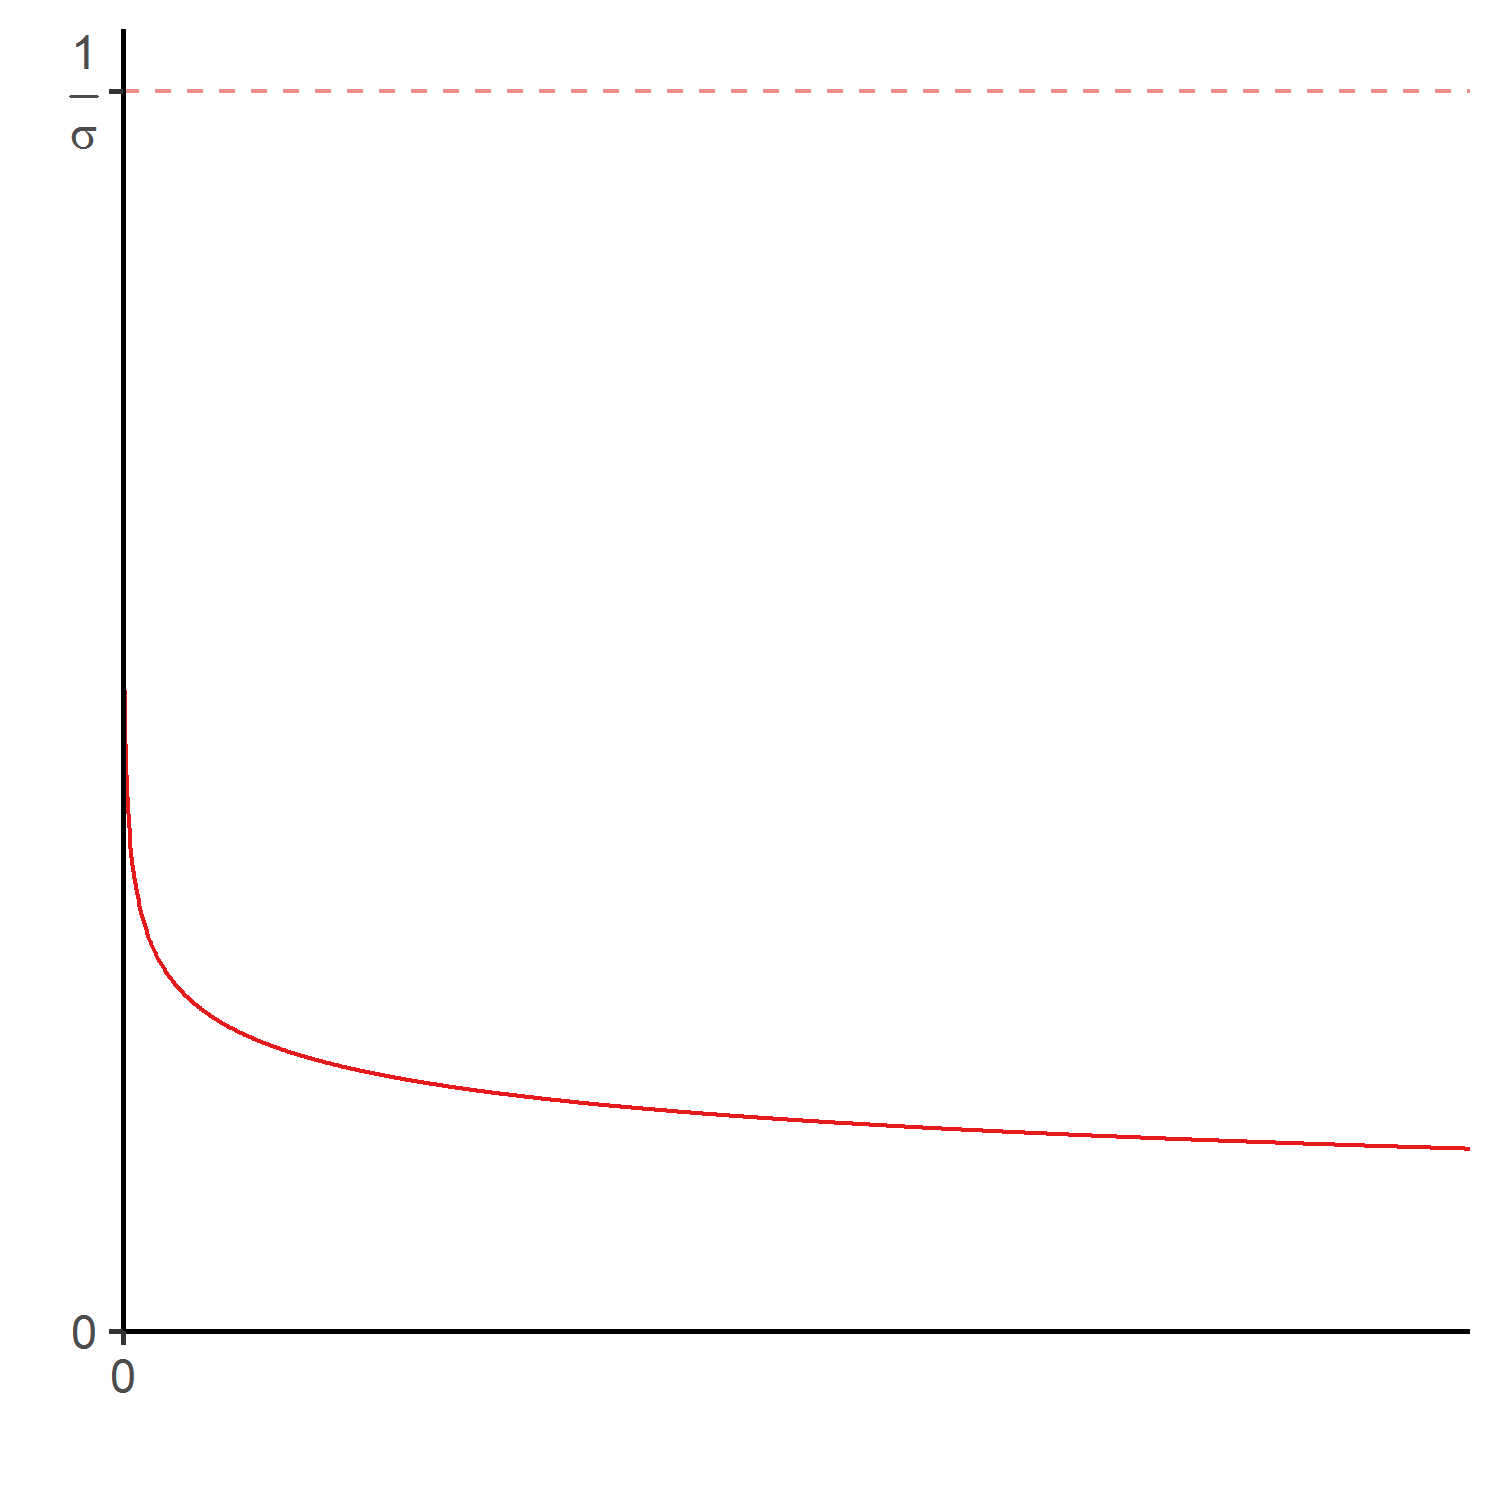
\includegraphics[width=1\linewidth]{Figures/graph_2} 
					\caption{$ \sigma \in (0.5, 1)$} 
					\label{fig:graph_2} 
				\end{subfigure}
				%%%
				\begin{subfigure}[t]{0.32\linewidth}
					\centering
					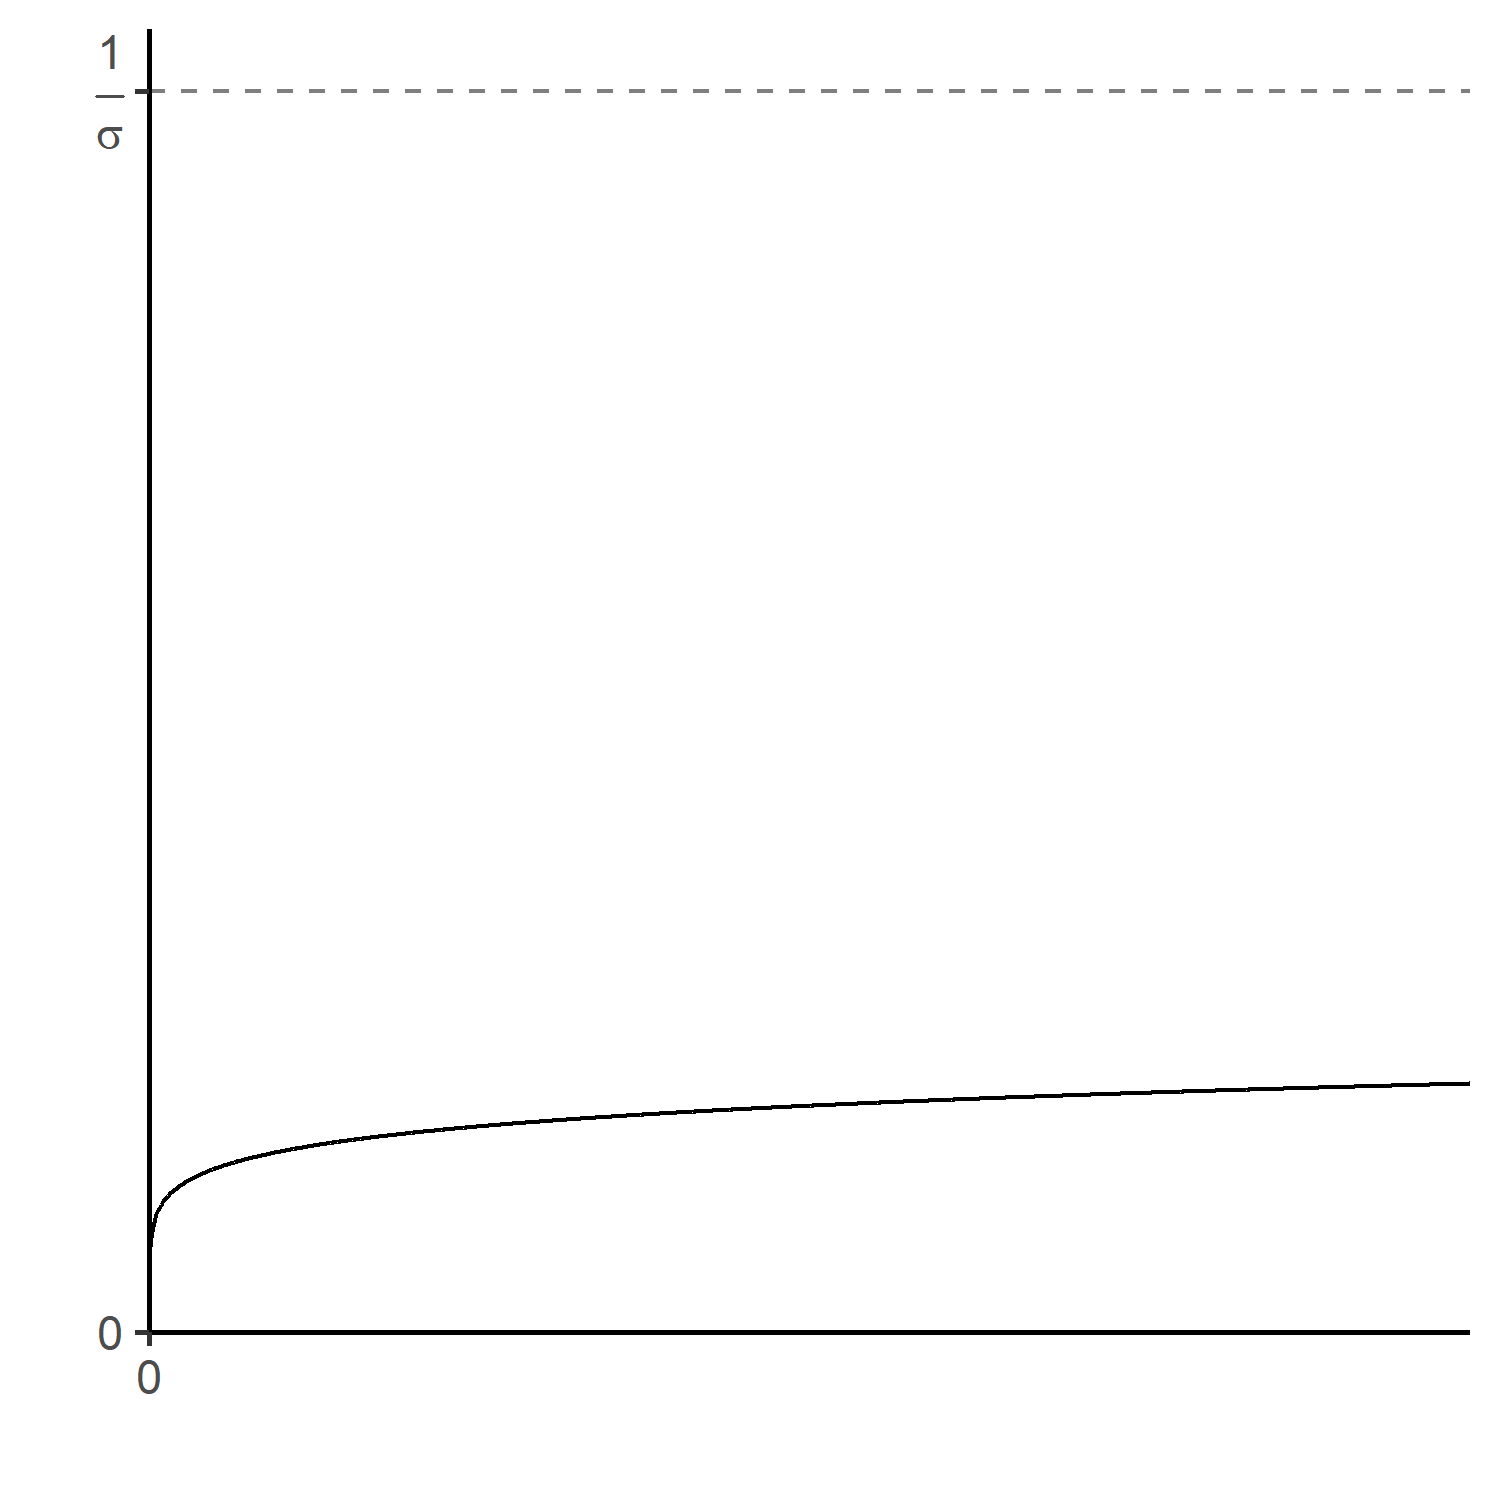
\includegraphics[width=1\linewidth]{Figures/graph_3} 
					\caption{$\sigma>1$} 
					\label{fig:graph_3} 
				\end{subfigure}
			\end{figure}
			\hyperlink{captolab<1>}{\beamerreturnbutton{Return}}
		\end{frame}
		\begin{frame}[label = leon]\frametitle{Production and labor share under biased technical change}
			\begin{itemize}
				\item Normalized CES production function :
				\begin{equation*}
					Y_t = A\left[\left(E_t^K K_t\right)^{\frac{\sigma - 1}{\sigma}} + \left(E_t^L L_t\right)^{\frac{\sigma - 1}{\sigma}}\right]^{\frac{\sigma}{\sigma - 1}}
				\end{equation*}
				\item Linear growth rates of efficiency levels : $E_t^i = E_0^i e^{a_i(t-t_0)}$
				\item Same fixed point : $ \begin{cases}
				E_0^K &= \frac{Y_0}{K_0}\left(\frac{1}{\phi_0}\right)^{\frac{\sigma}{\sigma - 1}}\\
				E_0^L &= \frac{Y_0}{L_0}\left(\frac{1}{1-\phi_0}\right)^{\frac{\sigma}{\sigma - 1}}
				\end{cases}$
				\item Labor share :
				\begin{equation*}
					\theta_t = \frac{w_t L_t}{Y_t} = \left[  1 + \frac{\phi_0}{1-\phi_0}\left( \frac{K_t}{L_t} \frac{L_0}{K_0} e^{(a_K - a_L)(t-t_0)}\right)^{\frac{\sigma - 1}{\sigma}}\right]^{-1}
				\end{equation*}
			\end{itemize}
			\hyperlink{paraminit<1>}{\beamerreturnbutton{Return}}
		\end{frame}
		\begin{frame}\frametitle{Estimation of the Capital-Labor elasticity of substitution}
			\begin{itemize}
				\item Identification of $\sigma$ following the methodology of León-Ledesma, McAdam \& Willman (2010)
				\vspace{1em}
				\item Under a normalized CES production function with biased technical change, the \textbf{Capital-to-Labor income ratio} is :
				\begin{equation*}
				\Theta	_t = \frac{\phi_0}{1-\phi_0}\left( \tilde{k}_t ~ e^{(a_K - a_L)(t-t_0)}\right)^{\frac{\sigma - 1}{\sigma}}
				\end{equation*}
				\item Rewriting the equation and taking logs :
				\begin{equation*}
				\ln \tilde{k}_t = \pi_0 - \frac{\sigma}{1-\sigma} \ln \Theta_t + (a_L - a_K)(t-t_0)
				\end{equation*}
				% where $\pi_0 = \frac{\sigma}{\sigma - 1}\ln\left(\frac{1-\phi_0}{\phi_0}\right)$
			\end{itemize}
			\hyperlink{paraminit<1>}{\beamerreturnbutton{Return}}
		\end{frame}
		\begin{frame}
			\begin{itemize}
				\item Balanced panel data on 4 countries over the period 1970-2010 from the PWT 9.0
			\end{itemize}
			\vspace{1em}
			\begin{itemize}
				\item Estimated equation : $ \ln \tilde{k}_{it} = \pi_{0i} + \pi_{1i} \ln \Theta_{it} + \pi_{2i}(t-t_0)$
			\end{itemize}
			\vspace{-1em}
			\begin{center}
			\resizebox{11cm}{!}{\begin{threeparttable}
	\caption{Estimation of the capital-labor elasticity of substitution.}
	\label{tab:sigma_est}
	\begin{tabular}{c D{.}{.}{-3} D{.}{.}{-3} D{.}{.}{-3} D{.}{.}{-3}}
		\multicolumn{5}{c}{France}  \\ \hline \hline \\ [-1ex]
		$\alpha$ 							& 1.460^{***} 	& 1.130^{***}	& 1.445^{***}	& 1.081^{***}	\\
											& (0.056)		& (0.040)		& (0.176)		& (0.039)		\\
		$\frac{1-\sigma}{\sigma}$ 			& -0.374^{***} 	& -0.614^{***}	& -0.360^{**}	& -0.273 		\\
											& (0.027)		& (0.055)		& (0.152)		& (0.184)			\\
		$\frac{1-\sigma}{\sigma}(a_K-a_L)$ 	& 				&				& -0.000		& -0.007^{*}	\\
											& 				&				& (0.005)		& (0.004)		\\ [1ex] \hline \\ [-1ex]
		Biased technical change 			& \multicolumn{1}{c}{No} & \multicolumn{1}{c}{No} & \multicolumn{1}{c}{Yes} & \multicolumn{1}{c}{Yes} \\
		Hours worked correction 			& \multicolumn{1}{c}{No} & \multicolumn{1}{c}{Yes} & \multicolumn{1}{c}{No} & \multicolumn{1}{c}{Yes} \\ [1ex] \hline \\ [-1ex]		
		$\sigma$ 							& 1.598			& 2.593			& 1.564			& 1.375		\\ [1ex]
		\hline \hline
	\end{tabular}
	\begin{tabular}{c D{.}{.}{-3} D{.}{.}{-3} D{.}{.}{-3} D{.}{.}{-3}}
		\multicolumn{5}{c}{United States} \\ \hline \hline \\ [-1ex]
		$\alpha$ 							& 0.761^{***}	& 0.636^{***}	& 0.535^{***}	& 0.643^{***} \\
											& (0.058)		& (0.017)		& (0.202)		& (0.018) \\
		$\frac{1-\sigma}{\sigma}$ 			& -0.130^{***}	& -0.177^{***}	& 0.111			& 0.155 \\
											& (0.044)		& (0.059)		& (0.211)		& (0.365) \\
		$\frac{1-\sigma}{\sigma}(a_K-a_L)$ 	&				&				& -0.004		& -0.004 \\
											&				&				& (0.003)		& (0.005) \\ [1ex] \hline \\ [-1ex]
		Biased technical change 			& \multicolumn{1}{c}{No} & \multicolumn{1}{c}{No} & \multicolumn{1}{c}{Yes} & \multicolumn{1}{c}{Yes} \\
		Hours worked correction 			& \multicolumn{1}{c}{No} & \multicolumn{1}{c}{Yes} & \multicolumn{1}{c}{No} & \multicolumn{1}{c}{Yes} \\ [1ex] \hline \\ [-1ex]		
		$\sigma$ 							& 1.150			& 1.215			& 0.900			& 0.866\\ [1ex]
		\hline \hline
	\end{tabular}
	
	\begin{tablenotes}
		{\footnotesize 
			\item \textit{Note :} $^{*}$p$<$0.1; $^{**}$p$<$0.05; $^{***}$p$<$0.01. Robust standard errors in parenthesis.
		}
	\end{tablenotes}
\end{threeparttable}}
			\end{center}
			\hyperlink{paraminit<1>}{\beamerreturnbutton{Return}}
		\end{frame}
	

	
\end{document}